\documentclass[a4paper, 11pt, oneside, polutonikogreek, german]{article}
\usepackage[utf8]{inputenc}
\usepackage[T1]{fontenc}
\usepackage{ebgaramond}

% Load encoding definitions (after font package)

\usepackage{textalpha}
\usepackage{listings}
\lstset{basicstyle=\ttfamily}

\usepackage[dvipsnames]{xcolor}
\usepackage{eso-pic,graphicx}
\usepackage[top=80mm, bottom=82mm, outer=80mm, inner=49mm]{geometry}
\setlength{\columnsep}{90pt}

% Babel package:
\usepackage[greek]{babel}

% With XeTeX$\$LuaTeX, load fontspec after babel to use Unicode
% fonts for Latin script and LGR for Greek:
\ifdefined\luatexversion \usepackage{fontspec}\fi
\ifdefined\XeTeXrevision \usepackage{fontspec}\fi

% "Lipsiakos" italic font `cbleipzig`:
\newcommand*{\lishape}{\fontencoding{LGR}\fontfamily{cmr}%
		       \fontshape{li}\selectfont}
\DeclareTextFontCommand{\textli}{\lishape}

\usepackage{setspace}
\onehalfspacing

\usepackage{booktabs}
\setlength{\emergencystretch}{3em}
\usepackage{fancyhdr}
\usepackage{microtype}
\definecolor{darkLapis}{RGB}{27,41,75}

% change color of text, example replace all \color{Goldenrod} with \color{lightgray}

\makeatletter % change only the display of \thepage, but not \thepage itself:
\patchcmd{\ps@plain}{\thepage}{\bfseries\large\color{darkLapis}{\thepage}}{}{}
\makeatother

\color{darkLapis}

\begin{document}
\bfseries
\AddToShipoutPictureBG{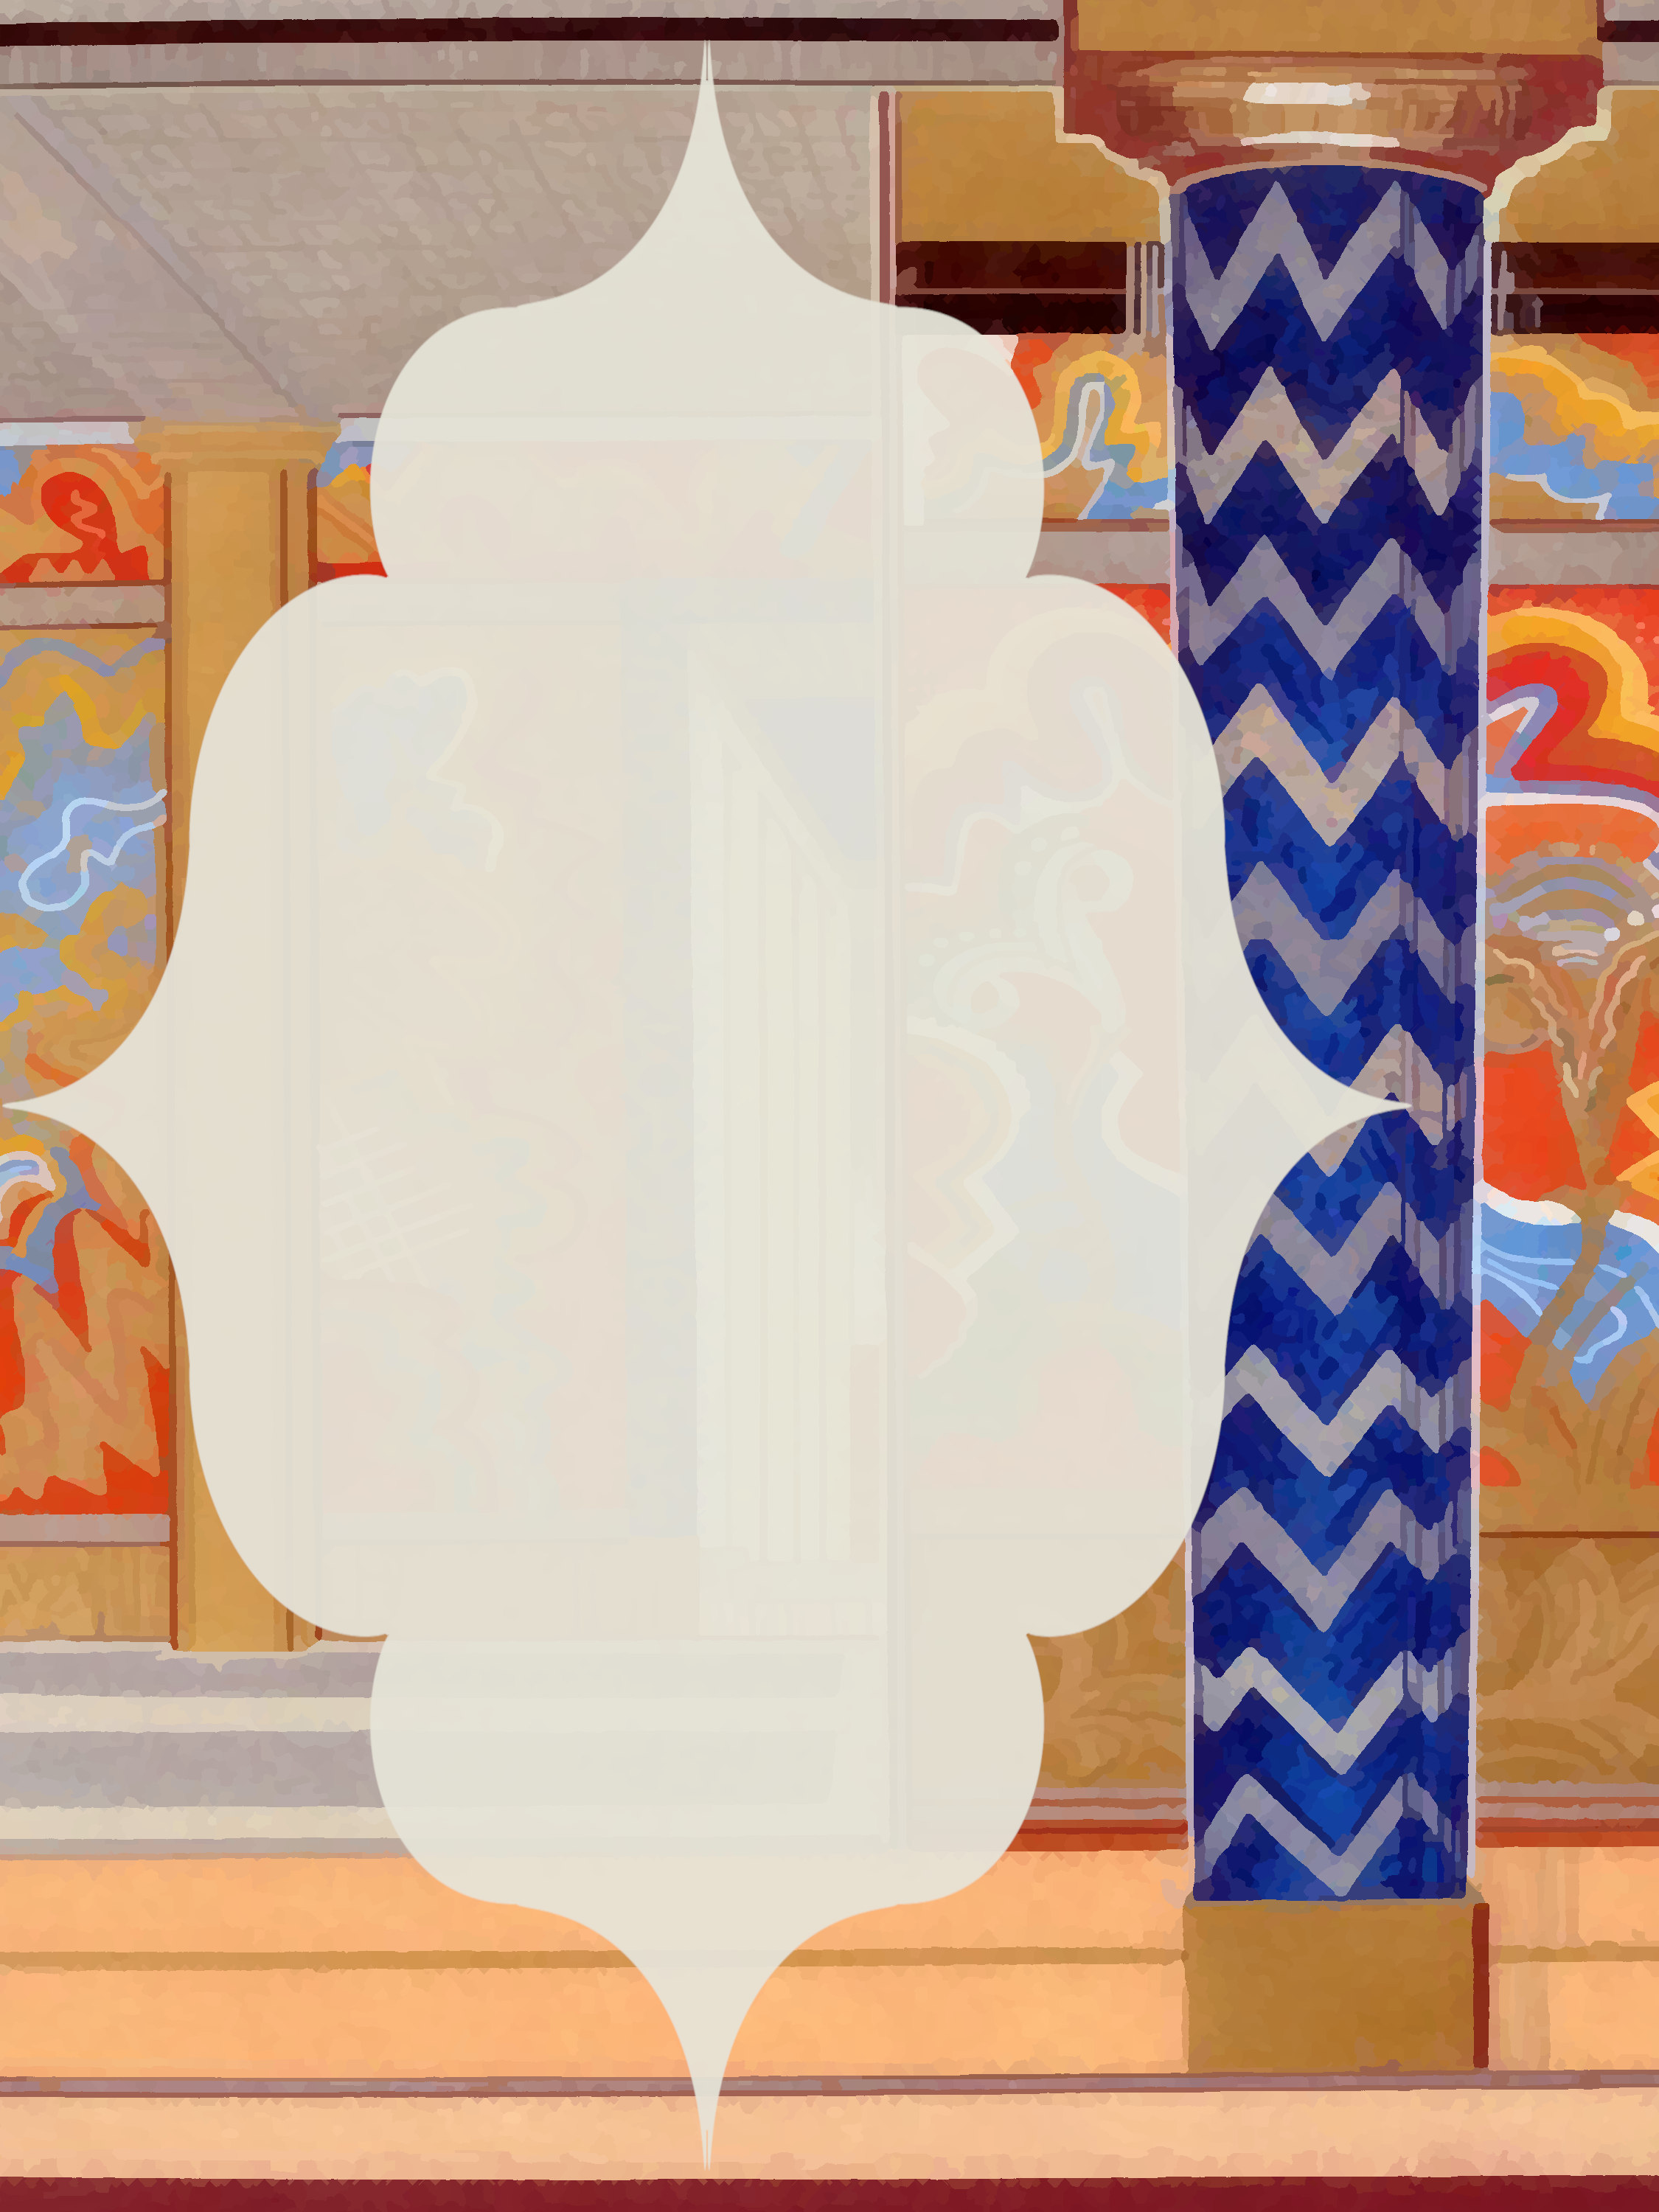
\includegraphics[width=\paperwidth,height=\paperheight]{greek3.jpeg}}
\begin{titlepage} % Suppresses headers and footers on the title page
	\centering % Centre everything on the title page
	%\scshape % Use small caps for all text on the title page

	%------------------------------------------------
	%	Title
	%------------------------------------------------

	\rule{\textwidth}{1.6pt}\vspace*{-\baselineskip}\vspace*{2pt} % Thick horizontal rule
	\rule{\textwidth}{0.4pt} % Thin horizontal rule
	
	\vspace{1\baselineskip} % Whitespace above the title
	
	{\scshape\Huge Περι της Συρίης Θεου}
	
	\vspace{1\baselineskip} % Whitespace above the title

	\rule{\textwidth}{0.4pt}\vspace*{-\baselineskip}\vspace{3.2pt} % Thin horizontal rule
	\rule{\textwidth}{1.6pt} % Thick horizontal rule
	
	\vspace{1\baselineskip} % Whitespace after the title block
	
	%------------------------------------------------
	%	Subtitle
	%------------------------------------------------
	
	{\scshape \Large Λουκιανός}
 
        \vspace{0.5\baselineskip}
	
	\vspace*{1\baselineskip} % Whitespace under the subtitle
	
        {\scshape \normalsize } % Subtitle or further description

	%------------------------------------------------
	%	Editor(s)
	%------------------------------------------------
        \vspace*{\fill}    

	\vspace{1\baselineskip}

	{\small\scshape 1852}
	
	{\small\scshape{Sumptibus et Typis B. G. Teubneri}}
	
	\vspace{0.5\baselineskip} % Whitespace after the title block

        \scshape Internet Archive Online Edition% Publication year
    
	{\scshape\small Creative Commons Αναφορά-Μη Εμπορική Χρήση 4.0} % Publisher
\end{titlepage}
\setlength{\parskip}{1mm plus1mm minus1mm}
\clearpage
\large
%\tableofcontents
%\clearpage
\paragraph{}
\textbf{1.} Ἔστιν ἐν Συρίῃ πόλις οὐ πολλὸν ἀπὸ τοῦ Εὐφρήτεω ποταμοῦ, καλέεται δὲ Ἱρὴ καὶ ἔστιν ἱρὴ τῆς Ἥρης τῆς Ἀσσυρίης. δοκέει δέ μοι, τόδε τὸ οὔνομα οὐκ ἅμα τῇ πόλι οἰκεομένῃ ἐγένετο, ἀλλὰ τὸ μὲν ἀρχαῖον ἄλλο ἦν · μετὰ δὲ σφίσι τῶν ἱρῶν μεγάλων γιγνομένων ἐς τόδε ἡ ἐπωνυμίη ἀπίκετο. περὶ ταύτης ὦν τῆς πόλιος ἔρχομαι ἐρέων ὁκόσα ἐν αὐτῇ ἐστιν · ἐρέω δὲ καὶ νόμους, τοῖσιν ἐς τὰ ἱρὰ χρέονται, καὶ πανηγύριας τὰς ἄγουσι καὶ θυσίας τὰς ἐπιτελέουσιν. ἐρέω δὲ ὁκόσα καὶ περὶ τῶν τὸ ἱρὸν εἱσαμένων μυθολογέουσι, καὶ τὸν νηὸν ὅκως ἐγένετο. γράφω δὲ Ἀσσύριος ἐών, καὶ τῶν ἀπηγέομαι τὰ μὲν αὐτοψίῃ ἔμαθον, τὰ δὲ παρὰ τῶν ἱρέων ἐδάην, ὁκόσα ἐόντα ἐμεῦ πρεσβύτερα ἐγὼ ἱστορέω.

\textbf{2.} Πρῶτοι μὲν ῶν ἀνθρώπων, τῶν ἡμεῖς ἴδμεν, Αἰγύπτιοι λέγονται θεῶν τε ἐννοίην λαβεῖν καὶ ἱρὰ εἴσασθαι καὶ τεμένεα καὶ πανηγύριας ἀποδέξαι. πρῶτοι δὲ καὶ οὐνόματα ἱρὰ ἔγνωσαν καὶ λόγους ἱροὺς ἔλεξαν. μετὰ δὲ οὐ πολλοστῷ χρόνῳ παρ ᾽ Αἰγυπτίων λόγον Ἀσσύριοι ἐς θεοὺς ἤκουσαν καὶ ἱρὰ καὶ νηοὺς ἤγειραν, ἐν τοῖσι καὶ ἀγάλματα ἔθεντο καὶ ξόανα ἐστήσαντο. \textbf{3.} τὸ δὲ παλαιὸν καὶ παρ ᾽ Αἰγυπτίοισιν ἀξόανοι νηοὶ ἔσαν. καὶ ἔστιν ἱρὰ καὶ ἐν Συρίῃ οὐ παρὰ πολὺ τοῖς Αἰγυπτίοισιν ἰσοχρονέοντα, τῶν ἐγὼ πλεῖστα ὄπωπα · τό γε τοῦ Ἡρακλέος τὸ ἐν Τύρῳ, οὐ τούτου τοῦ Ἡρακλέος, τὸν Ἕλληνες ἀείδουσιν, ἀλλὰ τὸν ἐγὼ λέγω, πολλὸν ἀρχαιότερος, καὶ Τύριος ἥρως ἐστίν. \textbf{4.} ἔνι δὲ καὶ ἄλλο ἱρὸν ἐν Φοινίκῃ μέγα, τὸ Σιδώνιοι ἔχουσιν, ὡς μὲν αὐτοὶ λέγουσιν, Ἀστάρτης ἐστίν · Ἀστάρτην δ ᾽ ἐγὼ δοκέω Σεληναίην ἔμμεναι · ὡς δέ μοί τις τῶν ἱρέων ἀπηγέετο, Εὐρώπης ἐστὶ τῆς Κάδμου ἀδελφεῆς. ταύτην δ ᾽ ἐοῦσαν Ἀγήνορος τοῦ βασιλῆος θυγατέρα, ἐπειδή τε ἀφανὴς ἐγεγόνεεν, οἱ Φοίνικες τῷ νηῷ ἐτιμήσαντο καὶ λόγον ἱρὸν ἐπ ᾽ αὐτῇ ἔλεξαν, ὅτι ἐοῦσαν καλὴν Ζεὺς ἐπόθεε καὶ τὸ εἶδος εἰς ταῦρον ἀμειψάμενος ἥρπασε, καί μιν ἐς Κρήτην φέρων ἀπίκετο. τάδε μὲν καὶ τῶν ἄλλων Φοινίκων ἤκουον, καὶ τὸ νόμισμα, τῷ Σιδώνιοι χρέονται, τὴν Εὐρώπην ἐφεζομένην ἔχει τῷ ταύρῳ τῷ Διί · τὸν δὲ νηὸν οὐκ ὁμολογέουσιν Εὐρώπης ἔμμεναι. \textbf{5.} ἔχουσι δὲ καὶ ἄλλο Φοίνικες ἱρόν, οὐκ Ἀσσύριον, ἀλλ ᾽ Αἰγύπτιον, τὸ ἐξ Ἡλίου πόλιος ἐς τὴν Φοινίκην ἀπίκετο. ἐγὼ μέν μιν οὐκ ὄπωπα, μέγα δὲ καὶ τόδε καὶ ἀρχαῖόν ἐστιν. \textbf{6.} εἶδον δὲ καὶ ἐν Βύβλῳ μέγα ἱρὸν Ἀφροδίτης Βυβλίης, ἐν τῷ καὶ τὰ ὄργια ἐς Ἄδωνιν ἐπιτελέουσιν · ἐδάην δὲ καὶ τὰ ὄργια. λέγουσι γὰρ δὴ ὦν τὸ ἔργον τὸ ἐς Ἄδωνιν ὑπὸ τοῦ συὸς ἐν τῇ χώρῃ τῇ σφετέρῃ γενέσθαι καὶ μνήμην τοῦ πάθεος τύπτονταί τε ἑκάστου ἔτεος καὶ θρηνέουσι καὶ τὰ ὄργια ἐπιτελέουσιν καὶ σφίσι μεγάλα πένθεα ἀνὰ τὴν χώρην ἵσταται. ἐπεὰν δὲ ἀποτύψωνταί τε καὶ ἀποκλαύσωνται, πρῶτα μὲν καταγίζουσι τῷ Ἀδώνιδι ὅκως ἐόντι νέκυι, μετὰ δὲ τῇ ἑτέρῃ ἡμέρῃ ζώειν τέ μιν μυθολογέουσι καὶ ἐς τὸν ἠέρα πέμπουσι καὶ τὰς κεφαλὰς ξυρέονται ὅκως Αἰγύπτιοι ἀποθανόντος Ἄπιος. γυναικῶν δὲ ὁκόσαι οὐκ ἐθέλουσι ξυρέεσθαι, τοιήνδε ζημίην ἐκτελέουσιν · ἐν μιῇ ἡμέρῃ ἐπὶ πρήσι τῆς ὥρης ἵστανται, ἡ δὲ ἀγορὴ μούνοισι ξείνοισι παρακέεται καὶ ὁ μισθὸς ἐς τὴν Ἀφροδίτην θυσίη γίγνεται. \textbf{7.} εἰσὶ δὲ ἔνιοι Βυβλίων, οἳ λέγουσι παρὰ σφίσι τεθάφθαι τὸν Ὄσιριν τὸν Αἰγύπτιον, καὶ τὰ πένθεα καὶ τὰ ὄργια οὐκ ἐς τὸν Ἄδωνιν, ἀλλ ᾽ ἐς τὸν Ὄσιριν πάντα πρήσσεσθαι. ἐρέω δὲ ὁκόθεν καὶ τάδε πιστὰ δοκέουσι. κεφαλὴ ἑκάστου ἔτεος ἐξ Αἰγύπτου ἐς τὴν Βύβλον ἀπικνέεται πλώουσα τὸν μεταξὺ πλόον ἑπτὰ ἡμερέων, καί μιν οἱ ἄνεμοι φορέουσι θείῃ ναυτιλίῃ · τρέπεται δὲ οὐδαμά, ἀλλ ᾽ ἐς μούνην τὴν Βύβλον ἀπικνέεται. καὶ ἔστι τὸ σύμπαν θωῦμα. καὶ τοῦτο ἑκάστου ἔτεος γίγνεται, τὸ καὶ ἐμεῦ παρεόντος ἐν Βύβλῳ ἐγένετο · καὶ τὴν κεφαλὴν ἐθεησάμην Βυβλίνην. \textbf{8.} ἔνι δὲ καὶ ἄλλο θωῦμα ἐν τῇ χώρῃ τῇ Βυβλίνῃ, ποταμὸς ἐκ τοῦ Λιβάνου τοῦ οὔρεος ἐς τὴν ἅλα ἐκδιδοῖ · οὔνομα τῷ ποταμῷ Ἄδωνις ἐπικέεται. ὁ δὲ ποταμὸς ἑκάστου ἔτεος αἱμάσσεται καὶ τὴν χροιὴν ὀλέσας ἐσπίπτει ἐς τὴν θάλασσαν καὶ φοινίσσει τὸ πολλὸν τοῦ πελάγεος καὶ σημαίνει τοῖς Βυβλίοις τὰ πένθεα. μυθέονται δὲ ὅτι ταύτῃσι τῇσιν ἡμέρῃσιν ὁ Ἄδωνις ἀνὰ τὸν Λίβανον τιτρώσκεται καὶ τὸ αἷμα ἐς τὸ ὕδωρ ἐρχόμενον ἀλλάσσει τὸν ποταμὸν καὶ τῷ ῥόῳ τὴν ἐπωνυμίην διδοῖ. ταῦτα μὲν οἱ πολλοὶ λέγουσιν. ἐμοὶ δέ τις ἀνὴρ Βύβλιος ἀληθέα δοκέων λέγειν ἑτέρην ἀπηγέετο τοῦ πάθεος αἰτίην. ἔλεγε δὲ ὧδε · ὁ Ἄδωνις ὁ ποταμός, ὦ ξεῖνε, διὰ τοῦ Λιβάνου ἔρχεται · ὁ δὲ Λίβανος κάρτα ξανθόγεώς ἐστιν · ἄνεμοι ὦν τρηχέες ἐκείνῃσι τῇσιν ἡμέρῃσιν ἱστάμενοι τὴν γῆν τῷ ποταμῷ ἐπιφέρουσι ἐοῦσαν ἐς τὰ μάλιστα μιλτώδεα, ἡ δὲ γῆ μιν αἱμώδεα τίθησι · καὶ τοῦδε τοῦ πάθεος οὐ τὸ αἷμα, τὸ λέγουσιν, ἀλλ ᾽ ἡ χώρη αἰτίη. ὁ μέν μοι Βύβλιος τοσαῦτα ἀπηγέετο · εἰ δὲ ἀτρεκέως ταῦτα ἔλεγεν, ἐμοὶ μὲν δοκέει κάρτα θείη καὶ τοῦ ἀνέμου ἡ συντυχίη. \textbf{9.} ἀνέβην δὲ καὶ ἐς τὸν Λίβανον ἐκ Βύβλου, ὁδὸν ἡμέρης, πυθόμενος αὐτόθι ἀρχαῖον ἱρὸν Ἀφροδίτης ἔμμεναι, τὸ Κινύρης εἵσατο, καὶ εἶδον τὸ ἱρὸν καὶ ἀρχαῖον ἦν. τάδε μέν ἐστι τὰ ἐν τῇ Συρίῃ ἀρχαῖα καὶ μεγάλα ἱρά. \textbf{10.} τοσούτων δὲ ἐόντων ἐμοὶ δοκέει οὐδὲν τῶν ἐν τῇ ἱρῇ πόλι μεῖζον ἔμμεναι οὐδὲ νηὸς ἄλλος ἁγιώτερος οὐδὲ χώρη ἄλλη ἱροτέρη. ἔνι δὲ καὶ ἔργα ἐν αὐτῷ πολυτελέα καὶ ἀρχαῖα ἀναθήματα καὶ πολλὰ θωύματα καὶ ξόανα θεοπρεπέα, καὶ θεοὶ δὲ κάρτα αὐτοῖσιν ἐμφανέες · ἱδρώει γὰρ δὴ ὦν παρὰ σφίσι τὰ ξόανα καὶ κινέεται καὶ χρησμηγορέει · καὶ βοὴ δὲ πολλάκις ἐγένετο ἐν τῷ νηῷ κλεισθέντος τοῦ ἱροῦ, καὶ πολλοὶ ἤκουσαν. ναὶ μὴν καὶ ὄλβου πέρι ἐν τοῖσιν ἐγὼ οἶδα πρῶτόν ἐστι · πολλὰ γὰρ αὐτοῖσιν ἀπικνέεται χρήματα ἔκ τε Ἀραβίης καὶ Φοινίκων καὶ Βαβυλωνίων καὶ ἄλλα ἐκ Καππαδοκίης, τὰ δὲ καὶ Κίλικες φέρουσι, τὰ δὲ Ἀσσύριοι. εἶδον δὲ ἐγὼ καὶ τὰ ἐν τῷ νηῷ λάθρῃ ἀποκέαται, ἐσθῆτα πολλὴν καὶ ἄλλα ὁκόσα ἐς ἄργυρον ἢ ἐς χρυσὸν ἀποκέκριται · ὁρταὶ μὲν γὰρ καὶ πανηγύριες οὐδαμοῖσιν ἄλλοισιν ἀνθρώπων τοσαίδε ἀποδεδέχαται. \textbf{11.} ἱστορέοντι δέ μοι ἐτέων πέρι, ὁκόσα τῷ ἱρῷ ἐστι, καὶ τὴν θεὸν αὐτοὶ ἥντινα δοκέουσι, πολλοὶ λόγοι ἐλέγοντο, τῶν οἱ μὲν ἱροί, οἱ δὲ ἐμφανέες, οἱ δὲ κάρτα μυθώδεες, καὶ ἄλλοι βάρβαροι, οἱ μὲν τοῖσιν Ἕλλησιν ὁμολογέοντες, τοὺς ἐγὼ πάντας μὲν ἐρέω, δέκομαι δὲ οὐδαμά. \textbf{12.} οἱ μὲν ὦν πολλοὶ Δευκαλίωνα τὸν Σισύθεα τὸ ἱρὸν εἵσασθαι λέγουσι, τοῦτον Δευκαλίωνα, ἐπὶ τοῦ τὸ πολλὸν ὕδωρ ἐγένετο. Δευκαλίωνος δὲ πέρι λόγον ἐν Ἕλλησιν ἤκουσα, τὸν Ἕλληνες ἐπ ᾽ αὐτῷ λέγουσιν. ὁ δὲ μῦθος ὧδε ἔχει · ἥδε ἡ γενεὴ οἱ νῦν ἄνθρωποι οὐ πρῶτοι ἐγένοντο, ἀλλ ᾽ ἐκείνη μὲν ἡ γενεὴ πάντες ὤλοντο. οὗτοι δὲ γένεος τοῦ δευτέρου εἰσί, τὸ αὖτις ἐκ Δευκαλίωνος ἐς πληθὺν ἀπίκετο. ἐκείνων δὲ πέρι τῶν ἀνθρώπων τάδε μυθέονται · ὑβρισταὶ κάρτα ἐόντες ἀθέμιστα ἔργα ἔπρησσον, οὔτε γὰρ ὅρκια ἐφύλασσον οὔτε ξείνους ἐδέκοντο οὔτε ἱκετέων ἠνείχοντο, ἀντ ᾽ ὧν σφίσιν ἡ μεγάλη συμφορὴ ἀπίκετο. αὐτίκα ἡ γῆ πολλὸν ὕδωρ ἐκδιδοῖ καὶ ὄμβροι μεγάλοι ἐγένοντο καὶ οἱ ποταμοὶ κατέβησαν μέζονες καὶ ἡ θάλασσα ἐπὶ πολλὸν ἀνέβη, ἐς ὃ πάντα ὕδωρ ἐγένοντο καὶ πάντες ὤλοντο, Δευκαλίων δὲ μοῦνος ἀνθρώπων ἐλίπετο ἐς γενεὴν δευτέρην εὐβουλίης τε καὶ τοῦ εὐσεβέος εἵνεκα. ἡ δέ οἱ σωτηρίη ἥδε ἐγένετο · λάρνακα μεγάλην, τὴν αὐτὸς εἶχεν, ἐς ταύτην ἐσβιβάσας παῖδάς τε καὶ γυναῖκας ἑωυτοῦ ἐσέβη · ἐσβαίνοντι δέ οἱ ἀπίκοντο σύες καὶ ἵπποι καὶ λεόντων γένεα καὶ ὄφιες καὶ ἄλλα ὁκόσα ἐν γῇ νέμονται, πάντα ἐς ζεύγεα. ὁ δὲ πάντα ἐδέκετο, καί μιν οὐκ ἐσίνοντο, ἀλλὰ σφίσι μεγάλη διόθεν φιλίη ἐγένετο. καὶ ἐν μιῇ λάρνακι πάντες ἔπλευσαν, ἔστε τὸ ὕδωρ ἐπεκράτεε. τὰ μὲν Δευκαλίωνος πέρι Ἕλληνες ἱστορέουσι. \textbf{13.} τὸ δὲ ἀπὸ τούτου λέγεται λόγος ὑπὸ τῶν ἐν τῇ ἱρῇ πόλι μεγάλως ἄξιος θωυμάσαι, ὅτι ἐν τῇ σφετέρῃ χώρῃ χάσμα μέγα ἐγένετο καὶ τὸ σύμπαν ὕδωρ κατεδέξατο · Δευκαλίων δέ, ἐπεὶ τάδε ἐγένετο, βωμούς τε ἔθετο καὶ νηὸν ἐπὶ τῷ χάσματι Ἥρης ἅγιον ἐστήσατο. ἐγὼ δὲ καὶ τὸ χάσμα εἶδον, καὶ ἔστιν ὑπὸ τῷ νηῷ κάρτα μικρόν. εἰ μὲν ὦν πάλαι καὶ μέγα ἐὸν νῦν τοιόνδε ἐγένετο, οὐκ οἶδα · τὸ δὲ ἐγὼ εἶδον, μικρόν ἐστι. σῆμα δὲ τῆς ἱστορίης τόδε πρήσσουσι · δὶς ἑκάστου ἔτεος ἐκ θαλάσσης ὕδωρ ἐς τὸν νηὸν ἀπικνέεται. φέρουσι δὲ οὐκ ἱρέες μοῦνον, ἀλλὰ πᾶσα Συρίη καὶ Ἀραβίη, καὶ πέρηθεν τοῦ Εὐφρήτεω πολλοὶ ἄνθρωποι ἐς θάλασσαν ἔρχονται καὶ πάντες ὕδωρ φέρουσι, τὸ πρῶτα μὲν ἐν τῷ νηῷ ἐκχέουσι, μετὰ δὲ ἐς τὸ χάσμα κατέρχεται, καὶ δέκεται τὸ χάσμα μικρὸν ἐὸν ὕδατος χρῆμα πολλόν. τὰ δὲ ποιέοντες Δευκαλίωνα ἐν τῷ ἱρῷ τόνδε νόμον θέσθαι λέγουσι συμφορῆς τε καὶ εὐεργεσίης μνῆμα ἔμμεναι. ὁ μὲν ὦν ἀρχαῖος αὐτοῖσι λόγος ἀμφὶ τοῦ ἱροῦ τοιόσδε ἐστί. \textbf{14.} ἄλλοι δὲ Σεμίραμιν τὴν Βαβυλωνίην, τῆς δὴ πολλὰ ἔργα ἐν τῇ Ἀσίῃ ἐστί, ταύτην καὶ τόδε τὸ ἕδος εἵσασθαι νομίζουσιν, οὐκ Ἥρῃ δὲ εἵσασθαι, ἀλλὰ μητρὶ ἑωυτῆς, τῆς Δερκετὼ οὔνομα. Δερκετοῦς δὲ εἶδος ἐν Φοινίκῃ ἐθεησάμην, θέημα ξένον · ἡμισέη μὲν γυνή, τὸ δὲ ὁκόσον ἐκ μηρῶν ἐς ἄκρους πόδας ἰχθύος οὐρὴ ἀποτείνεται. ἡ δὲ ἐν τῇ ἱρῇ πόλι πᾶσα γυνή ἐστι. πίστιες δὲ τοῦ λόγου αὐτοῖσι κάρτα ἐμφανέες · ἰχθύας χρῆμα ἱρὸν νομίζουσι καὶ οὔκοτε ἰχθύων ψαύουσι, καὶ ὄρνιθας τοὺς μὲν ἄλλους σιτέονται, περιστερὴν δὲ μούνην οὐ σιτέονται, ἀλλὰ σφίσιν ἥδε ἱρή. τὰ δὲ γιγνόμενα δοκέει αὐτοῖσι ποιέεσθαι Δερκετοῦς καὶ Σεμιράμιος εἵνεκα, τὸ μέν, ὅτι Δερκετὼ μορφὴν ἰχθύος ἔχει, τὸ δέ, ὅτι τὸ Σεμιράμιος τέλος ἐς περιστερὴν ἀπίκετο. ἀλλ ᾽ ἐγὼ τὸν μὲν νηὸν ὅτι Σεμιράμιος ἔργον ἐστί, τάχα κου δέξομαι · Δερκετοῦς δὲ τὸ ἱρὸν ἔμμεναι οὐδαμὰ πείθομαι, ἐπεὶ καὶ παρ ᾽ Αἰγυπτίων ἐνίοισιν ἰχθύας οὐ σιτέονται, καὶ τάδε οὐ Δερκετοῖ χαρίζονται. \textbf{15.} ἔστι δὲ καὶ ἄλλος λόγος ἱρός, τὸν ἐγὼ σοφοῦ ἀνδρὸς ἤκουσα, ὅτι ἡ μὲν θεὴ Ῥέη ἐστί, τὸ δὲ ἱρὸν Ἄττεω ποίημα. Ἄττης δὲ γένος μὲν Λυδὸς ἦν, πρῶτος δὲ τὰ ὄργια τὰ ἐς Ῥέην ἐδιδάξατο. καὶ τὰ Φρύγες καὶ Λυδοὶ καὶ Σαμόθρᾳκες ἐπιτελέουσιν, Ἄττεω πάντα ἔμαθον · ὡς γάρ μιν ἡ Ῥέη ἔτεμε, βίου μὲν ἀνδρηίου ἀπεπαύσατο, μορφὴν δὲ θηλέην ἠμείψατο καὶ ἐσθῆτα γυναικηίην ἐνεδύσατο καὶ ἐς πᾶσαν γῆν φοιτέων ὄργιά τε ἐπετέλεε καὶ τὰ ἔπαθεν ἀπηγέετο καὶ Ῥέην ἤειδεν. ἐν  τοῖσι καὶ ἐς Συρίην ἀπίκετο. ὡς δὲ οἱ πέρην Εὐφρήτεω ἄνθρωποι οὔτε αὐτὸν οὔτε ὄργια ἐδέκοντο, ἐν τῷδε τῷ χώρῳ τὸ ἱρὸν ἐποιήσατο. σημήια δέ · ἡ θεὸς τὰ πολλὰ ἐς Ῥέην ἐπικνέεται. λέοντες γάρ μιν φέρουσι καὶ τύμπανον ἔχει καὶ ἐπὶ τῇ κεφαλῇ πυργοφορέει, ὁκοίην Ῥέην Λυδοὶ ποιέουσιν. ἔλεγε δὲ καὶ Γάλλων πέρι, οἵ εἰσιν ἐν τῷ ἱρῷ, ὅτι Γάλλοι Ἥρῃ μὲν οὐδαμά, Ῥέῃ δὲ τέμνονται καὶ Ἄττεα μιμέονται. τὰ δέ μοι εὐπρεπέα μὲν δοκέει ἔμμεναι, ἀληθέα δὲ οὔ · ἐπεὶ καὶ τῆς τομῆς ἄλλην αἰτίην ἤκουσα πολλὸν πιστοτέρην. \textbf{16.} ἁνδάνει δέ μοι τὰ λέγουσι τοῦ ἱροῦ πέρι τοῖσιν Ἕλλησιν τὰ πολλὰ ὁμολογέοντες, τὴν μὲν θεὸν Ἥρην δοκέοντες, τὸ δ ᾽ ἔργον Διονύσου τοῦ Σεμέλης ποίημα · καὶ γὰρ δὴ Διόνυσος ἐς Συρίην ἀπίκετο κείνην ὁδὸν τὴν ἦλθεν ἐπ ᾽ Αἰθιοπίην. καὶ ἔστι πολλὰ ἐν τῷ ἱρῷ Διονύσου ποιητέω σήματα, ἐν τοῖσι καὶ ἐσθῆτες βάρβαροι καὶ λίθοι Ἰνδοὶ καὶ ἐλεφάντων κέρεα, τὰ Διόνυσος ἐξ Αἰθιόπων ἤνεικε, καὶ φαλλοὶ δὲ ἑστᾶσιν ἐν τοῖσι προπυλαίοισι δύο κάρτα μεγάλοι, ἐπὶ τῶν ἐπίγραμμα τοιόνδε ἐπιγέγραπται, "`τούσδε φαλλοὺς Διόνυσος Ἥρῃ μητρυιῇ ἀνέθηκα."'

Ἐμοὶ μέν νυν καὶ τάδε ἀρκέει. ἐρέω δὲ καὶ ἄλλ ᾽ ὅ τι ἐστὶν ἐν τῷ νηῷ Διονύσου ὄργιον. φαλλοὺς Ἕλληνες Διονύσῳ ἐγείρουσιν, ἐπὶ τῶν καὶ τοιόνδε τι φέρουσιν, ἄνδρας μικροὺς ἐκ ξύλου πεποιημένους, μεγάλα αἰδοῖα ἔχοντας · καλέονται δὲ τάδε νευρόσπαστα. ἔστι δὲ καὶ τόδε ἐν τῷ ἱρῷ, ἐν δεξιῇ τοῦ νηοῦ κάθηται σμικρὸς ἀνὴρ χάλκεος ἔχων αἰδοῖον μέγα. \textbf{17.} τοσάδε μὲν ἀμφὶ τῶν οἰκιστέων τοῦ ἱροῦ μυθολογέουσιν. ἤδη δὲ ἐρέω καὶ τοῦ νηοῦ πέρι θέσιός τε ὅκως ἐγένετο καὶ ὅστις μιν ἐποιήσατο. λέγουσι τὸν νηὸν τὸν νῦν ἐόντα μὴ ἔμμεναι τὸν τὴν ἀρχὴν γεγενημένον, ἀλλ ᾽ ἐκεῖνον μὲν κατενεχθῆναι χρόνῳ ὕστερον, τὸν δὲ νῦν ἐόντα Στρατονίκης ἔμμεναι ποίημα, γυναικὸς τοῦ Ἀσσυρίων βασιλῆος. δοκέει δέ μοι ἡ Στρατονίκη ἐκείνη ἔμμεναι, τῆς ὁ πρόγονος ἠρήσατο, τὸν ἤλεγξε τοῦ ἰητροῦ ἐπινοίη · ὡς γάρ μιν ἡ συμφορὴ κατέλαβεν, ἀμηχανέων τῷ κακῷ αἰσχρῷ δοκέοντι κατ ᾽ ἡσυχίην ἐνόσεεν. ἔκειτο δὲ ἀλγέων οὐδέν, καί οἱ ἥ τε χροιὴ πάμπαν ἐτρέπετο καὶ τὸ σῶμα δι ᾽ ἡμέρης ἐμαραίνετο. ὁ δὲ ἰητρὸς ὡς εἶδέ μιν ἐς οὐδὲν ἐμφανὲς ἀρρωστέοντα, ἔγνω τὴν νοῦσον ἔρωτα ἔμμεναι. ἔρωτος δὲ ἀφανέος πολλὰ σημήια, ὀφθαλμοί τε ἀσθενέες καὶ φωνὴ καὶ χροιὴ καὶ δάκρυα. μαθὼν δὲ ταῦτα ἐποίεε · χειρὶ μὲν τῇ δεξιῇ ἔχε τοῦ νεηνίσκου τὴν καρδίην, ἐκάλεε δὲ τοὺς ἀνὰ τὴν οἰκίην πάντας · ὁ δὲ τῶν μὲν ἄλλων ἐσιόντων πάντων ἐν ἠρεμίῃ μεγάλῃ ἦν, ὡς δὲ ἡ μητρυιὴ ἀπίκετο, τήν τε χροιὴν ἠλλάξατο καὶ ἱδρώειν ἄρξατο καὶ τρόμῳ ἔχετο καὶ ἡ καρδίη ἀνεπάλλετο · τὰ δὲ γιγνόμενα ἐμφανέα τῷ ἰητρῷ τὸν ἔρωτα ἐποίεε. \textbf{18.} καί μιν ὧδε ἰήσατο · καλέσας τοῦ νεηνίσκου τὸν πατέρα κάρτα ὀρρωδέοντα, Ἥδε ἡ νοῦσος, ἔφη, τὴν ὁ παῖς ὅδε ἀρρωστέει, οὐ νοῦσός ἐστιν, ἀλλὰ ἀδικίη · ὅδε γάρ τοι ἀλγέει μὲν οὐδέν, ἔρως δέ μιν καὶ φρενοβλαβείη ἔχει. ἐπιθυμέει δὲ τῶν οὐδαμὰ τεύξεται, φιλέων γυναῖκα ἐμήν, τὴν ἐγὼ οὔτι μετήσομαι. ὁ μὲν ὦν τοιάδε σοφίῃ ἐψεύδετο. ὁ δὲ αὐτίκα ἐλίσσετο, Πρός τε σοφίης καὶ ἰητρικῆς μή μοι παῖδα ὀλέσῃς · οὐ γὰρ ἐθέλων ταύτῃ συμφορῇ ἔσχετο, ἀλλά οἱ ἡ νοῦσος ἀεκουσίη. τῷ σὺ μηδαμὰ ζηλοτυπέων πένθος ἐγεῖραι πάσῃ βασιληίῃ μηδὲ ἰητρὸς ἐὼν φθόνον προξενέειν ἰητρικῇ. ὁ μὲν ὧδε ἀγνὼς ἐὼν ἐδέετο. ὁ δέ μιν αὖτις ἀμείβετο, Ἀνόσια σπεύδεις γάμον ἐμὸν ἀπαιρεόμενος ἡδὲ ἰητρὸν ἄνδρα βιώμενος. σὺ δὲ κῶς ἂν αὐτὸς ἔπρηξας, εἴ τοι σὴν γυναῖκα ἐπόθεεν, ἐμεῦ τάδε δεόμενος ; ὁ δὲ πρὸς τάδε ἔλεγεν ὡς οὐδ ᾽ αὐτὸς ἄν κοτε γυναικὸς ἐφείσατο οὐδὲ παιδὶ σωτηρίης ἐφθόνεεν, εἰ καί οἱ μητρυιῆς ἐπεθύμεεν · οὐ γὰρ ὁμοίην συμφορὴν ἔμμεναι γαμετὴν ἢ παῖδα ὀλέσαι. ὡς δὲ τάδε ὁ ἰητρὸς ἤκουσε, Τί τοι, ἔφη, ἐμὲ λίσσεαι ; καὶ γάρ τοι σὴν γυναῖκα ποθέει · τὰ δὲ ἔλεγον ἐγώ, πάντα ἔην ψεύδεα. πείθεται μὲν τουτέοισι, καὶ τῷ μὲν παιδὶ λείπει καὶ γυναῖκα καὶ βασιληίην, αὐτὸς δὲ ἐς τὴν Βαβυλωνίην χώρην ἀπίκετο καὶ πόλιν ἐπὶ τῷ Εὐφρήτῃ ἐπώνυμον ἑωυτοῦ ἐποιήσατο, ἔνθα οἱ καὶ ἡ τελευτὴ ἐγένετο. ὧδε μὲν ὁ ἰητρὸς ἔρωτα ἔγνω τε καὶ ἰήσατο. \textbf{19.} ἥδε δὴ ὦν ἡ Στρατονίκη ἔτι τῷ προτέρῳ ἀνδρὶ συνοικέουσα ὄναρ τοιόνδε ἐθεήσατο, ὥς μιν ἡ Ἥρη ἐκέλευεν ἐγεῖραί οἱ τὸν ἐν τῇ ἱρῇ πόλι νηόν, εἰ δὲ ἀπειθέοι, πολλά οἱ καὶ κακὰ ἀπείλεεν. ἡ δὲ τὰ μὲν πρῶτα οὐδεμίην ὤρην ἐποιέετο, μετὰ δὲ ὥς μιν μεγάλη νοῦσος ἔλαβε, τῷ τε ἀνδρὶ τὴν ὄψιν ἀπηγήσατο καὶ τὴν Ἥρην ἱλάσκετο καὶ στήσειν τὸν νηὸν ὑπεδέξατο. καὶ αὐτίκα ὑγιέα γενομένην ὁ ἀνὴρ ἐς τὴν ἱρὴν πόλιν ἔπεμπε, σὺν δέ οἱ καὶ χρήματα καὶ στρατιὴν πολλήν, τοὺς μὲν οἰκοδομέειν, τοὺς δὲ καὶ τοῦ ἀσφαλέος εἵνεκα · καλέσας δέ τινα τῶν ἑωυτοῦ φίλων, νεηνίην κάρτα καλόν, τῷ οὔνομα ἦν Κομβάβος, Ἐγώ τοι, ἔφη, ὦ Κομβάβε, ἐσθλὸν ἐόντα φιλέω τε μάλιστα φίλων ἐμῶν καὶ πάμπαν ἐπαινέω σοφίης τε καὶ εὐνοίης τῆς ἐς ἡμέας, τὴν δὴ ἐπεδέξαο · νῦν δέ μοι χρειὼ μεγάλης πίστιος, τῷ σε θέλω γυναικὶ ἐμῇ ἑσπόμενον ἔργον τέ μοι ἐπιτελέσαι καὶ ἱρὰ τελέσαι καὶ στρατιῆς ἐπικρατέειν · σοὶ δὲ ἀπικομένῳ ἐξ ἡμέων τιμὴ μεγάλη ἔσσεται. πρὸς δὲ τάδε ὁ Κομβάβος αὐτίκα λίσσετο πολλὰ λιπαρέων μή μιν ἐκπέμπειν μηδὲ πιστεύειν οἱ τὰ πολλὸν ἑωυτοῦ μέζονα χρήματα καὶ γυναῖκα καὶ ἔργον ἱρόν · τὰ δὲ ὀρρώδεε μή κοτέ οἱ ζηλοτυπίη χρόνῳ ὑστέρῳ ἐς τὴν Στρατονίκην γένοιτο, τὴν μοῦνος ἀπάξειν ἔμελλεν. \textbf{20.} ὡς δὲ οὐδαμὰ ἐπείθετο, ὁ δὲ ἱκεσίης δευτέρης ἅπτεται δοῦναί οἱ χρόνον ἑπτὰ ἡμερέων, μετὰ δὲ ἀποστεῖλαί μιν τελέσαντά τι τῶν μάλιστα ἐδέετο. τυχὼν δὲ ῥηιδίως ἐς τὸν ἑωυτοῦ οἶκον ἀπικνέεται καὶ πεσὼν χαμᾶζε τοιάδε ὠδύρετο · ὢ δείλαιος, τί μοι ταύτης τῆς πίστιος ; τί δέ μοι ὁδοῦ, τῆς τέλος ἤδη δέρκομαι ; νέος μὲν ἐγὼ καὶ γυναικὶ καλῇ ἕψομαι. τὸ δέ μοι μεγάλη συμφορὴ ἔσσεται, εἰ μὴ ἔγωγε πᾶσαν αἰτίην κακοῦ ἀποθήσομαι. τῷ με χρῆν μέγα ἔργον ἀποτελέσαι, τό μοι πάντα φόβον ἰήσεται. τάδε εἰπὼν ἀτελέα ἑωυτὸν ἐποίεε, καὶ ταμὼν τὰ αἰδοῖα ἐς ἀγγήιον μικρὸν κατέθετο σμύρνῃ τε ἅμα καὶ μέλιτι καὶ ἄλλοισι θυώμασι καὶ ἔπειτα σφρηγῖδι τὴν ἐφόρεε σημηνάμενος τὸ τρῶμα ἰῆτο. μετὰ δὲ ὥς μιν ὁδοιπορέειν ἐδόκεεν, ἀπικόμενος ἐς τὸν βασιλῆα πολλῶν παρεόντων διδοῖ τε ἅμα τὸ ἀγγήιον καὶ λέγει ὧδε · Ὦ δέσποτα, τόδε μοι μέγα κειμήλιον ἐν τοῖσιν οἰκηίοισιν ἀπεκέετο, τὸ ἐγὼ κάρτα ἐπόθεον · νῦν δὲ ἐπεὶ μεγάλην ὁδὸν ἔρχομαι, παρὰ σοὶ τόδε θήσομαι. σὺ δέ μοι ἀσφαλέως ἔχειν · τόδε γάρ μοι χρυσοῦ βέλτερον, τόδε μοι ψυχῆς ἐμῆς ἀντάξιον. εὖτ ᾽ ἂν δὲ ἀπίκωμαι, σῶον αὖτις ἀποίσομαι. ὁ δὲ δεξάμενος ἑτέρῃ σφρηγῖδι ἐσημαίνετο καὶ τοῖσι ταμίῃσι φρουρέειν ἐνετείλατο. \textbf{21.} Κομβάβος μέν νυν τὸ ἀπὸ τοῦδε ἀσφαλέα ὁδὸν ἤνυεν · ἀπικόμενοι δὲ ἐς τὴν ἱρὴν πόλιν σπουδῇ τὸν νηὸν οἰκοδόμεον καὶ σφίσι τρία ἔτεα ἐν τῷ ἔργῳ ἐξεγένετο, ἐν τοῖσιν ἀπέβαινε τάπερ ὁ Κομβάβος ὀρρώδεεν · ἡ Στρατονίκη γὰρ χρόνον ἐπὶ πολλὸν συνόντα μιν ποθέειν ἄρχετο, μετὰ δέ οἱ καὶ κάρτα ἐπεμήνατο. καὶ λέγουσιν οἱ ἐν τῇ ἱρῇ πόλι τὴν Ἥρην τουτέων αἰτίην ἐθέλουσαν γενέσθαι, Κομβάβον ἐσθλὸν μὲν ἐόντα λαθέειν μηδαμά, Στρατονίκην δὲ τίσασθαι, ὅτι οὐ ῥηιδίως τὸν νηὸν ὑπέσχετο. \textbf{22.} ἡ δὲ τὰ μὲν πρῶτα ἐσωφρόνεε καὶ τὴν νοῦσον ἔκρυπτεν, ὡς δέ οἱ τὸ κακὸν μέζον ἡσυχίης ἐγένετο, ἐς ἐμφανὲς ἐτρύχετο κλαίεσκέ τε δι ᾽ ἡμέρης καὶ Κομβάβον ἀνεκαλέετο καί οἱ πάντα Κομβάβος ἦν. τέλος δὲ ἀμηχανέουσα τῇ συμφορῇ εὐπρεπέα ἱκεσίην ἐδίζητο. ἄλλῳ μὲν ὦν τὸν ἔρωτα ὁμολογέειν ἐφυλάσσετο, αὐτὴ δὲ ἐπιχειρέειν αἰδέετο. ἐπινοέει ὦν τοιάδε, οἴνῳ ἑωυτὴν μεθύσασα ἐς λόγους οἱ ἐλθεῖν · ἅμα δὲ οἴνῳ ἐσιόντι παρρησίη τε ἐσέρχεται καὶ ἡ ἀποτυχίη οὐ κάρτα αἰσχρή, ἀλλὰ τῶν πρησσομένων ἕκαστα ἐς ἀγνοίην ἀναχωρέει. ὡς δέ οἱ ἐδόκεε, καὶ ἐποίεε ταῦτα. καὶ ἐπεὶ ἐκ δείπνου ἐγένοντο, ἀπικομένη ἐς τὰ οἰκήια, ἐν τοῖσι Κομβάβος αὐλίζετο, λίσσετό τε καὶ γούνων ἅπτετο καὶ τὸν ἔρωτα ὡμολόγεεν · ὁ δὲ τόν τε λόγον ἀπηνέως ἀπεδέκετο καὶ τὸ ἔργον ἀναίνετο καί οἱ τὴν μέθην ἐνεκάλεεν. ἀπειλούσης δὲ μέγα τι κακὸν ἑωυτὴν ἐργάσασθαι, δείσας πάντα οἱ λόγον ἔφηνε καὶ πᾶσαν τὴν ἑωυτοῦ πάθην ἀπηγήσατο καὶ τὸ ἔργον ἐς ἐμφανὲς ἤνεικεν. ἰδοῦσα δὲ ἡ Στρατονίκη τὰ οὔκοτε ἔλπετο, μανίης μὲν ἐκείνης ἔσχετο, ἔρωτος δὲ οὐδαμὰ ἐλήθετο, ἀλλὰ πάντα οἱ συνεοῦσα ταύτην παραμυθίην ἐποιέετο ἔρωτος ἀπρήκτοιο. ἔστιν ὁ ἔρως οὗτος ἐν τῇ ἱρῇ πόλι καὶ ἔτι νῦν γίγνεται · γυναῖκες Γάλλων ἐπιθυμέουσιν καὶ γυναιξὶ Γάλλοι ἐπιμαίνονται, ζηλοτυπέει δὲ οὐδείς, ἀλλὰ σφίσι τὸ χρῆμα κάρτα ἱρὸν νομίζεται. \textbf{23.} τὰ δ ᾽ ὦν ἐν τῇ ἱρῇ πόλι ἀμφὶ τὴν Στρατονίκην οὐδαμὰ τὸν βασιλῆα λέληθεν, ἀλλὰ πολλοὶ ἀπικνεόμενοι κατηγόρεον καὶ τὰ γιγνόμενα ἀπηγέοντο. ἐπὶ τοῖσι περιαλγέων ἐξ ἀτελέος τοῦ ἔργου Κομβάβον μετεκάλεεν. ἄλλοι δὲ λέγουσι λόγον οὔτι ἀληθέα, τὴν Στρατονίκην, ἐπειδὴ ἀπέτυχε τῶν ἐδέετο, αὐτὴν γράψασαν ἐς τὸν ἄνδρα τοῦ Κομβάβου κατηγορέειν πείρην οἱ ἐπικαλέουσαν, καὶ τὸ Ἕλληνες Σθενεβοίης πέρι λέγουσι καὶ Φαίδρης τῆς Κνωσσίης, ταυτὶ καὶ Ἀσσύριοι ἐς Στρατονίκην μυθολογέουσιν. ἐγὼ μέν νυν οὔτε Σθενεβοίην πείθομαι οὔτε Φαίδρην τοιάδε ἐπιτελέσαι, εἰ τὸν Ἱππόλυτον ἀτρεκέως ἐπόθεε Φαίδρη. ἀλλὰ τὰ μὲν ἐχέτω ὅκως καὶ ἐγένετο. \textbf{24.} ὡς δὲ ἡ ἀγγελίη ἐς τὴν ἱρὴν πόλιν ἀπίκετο ἔγνω τε ὁ Κομβάβος τὴν αἰτίην, θαρσέων τε ἤιεν, ὅτι οἱ ἡ ἀπολογίη οἴκοι ἐλείπετο, καί μιν ἐλθόντα ὁ βασιλεὺς αὐτίκα μὲν ἔδησέ τε καὶ ἐν φρουρῇ ἔχε. μετὰ δὲ παρεόντων οἱ τῶν φίλων, οἳ καὶ τότε πεμπομένῳ τῷ Κομβάβῳ παρεγένοντο, παραγαγὼν ἐς μέσον κατηγορέειν ἄρχετο καί οἱ μοιχηίην τε καὶ ἀκολασίην προὔφερε · κάρτα δὲ δεινοπαθέων πίστιν τε καὶ φιλίην ἀνεκαλέετο λέγων τρισσὰ Κομβάβον ἀδικέειν μοιχόν τε ἐόντα καὶ ἐς πίστιν ὑβρίσαντα καὶ ἐς θεὸν ἀσεβέοντα, τῆς ἐν τῷ ἔργῳ τοιάδε ἔπρηξε · πολλοὶ δὲ παρεστεῶτες ἤλεγχον, ὅτι ἀναφανδὸν σφέας ἀλλήλοισι συνεόντας εἶδον. πᾶσι δὲ τέλος ἐδόκεεν αὐτίκα θνήσκειν Κομβάβον θανάτου ἄξια ἐργασμένον. \textbf{25.} ὁ δὲ τέως μὲν ἕστηκε λέγων οὐδέν · ἐπεὶ δὲ ἤδη ἐς τὸν φόνον ἤγετο, φθέγξατό τε καὶ τὸ κειμήλιον αἴτεε λέγων, ὡς ἀναιρέει μιν οὐκ ὕβριος οὐδὲ γάμων εἵνεκα, ἀλλ ᾽ ἐκείνων ἐπιθυμέων, τά οἱ ἀπιὼν παρεθήκατο. πρὸς τάδε ὁ βασιλεὺς καλέσας τὸν ταμίην ἐκέλευεν ἐνεῖκαι τά οἱ φρουρέειν ἔδωκεν · ὡς δὲ ἤνεικε, λύσας τὴν σφρηγῖδα ὁ Κομβάβος τά τε ἐνεόντα ἐπέδειξε καὶ ἑωυτὸν ὁκοῖα ἐπεπόνθεεν, ἔλεξέ τε, Ὦ βασιλεῦ, τάδε τοι ἐγὼ ὀρρωδέων, εὖτέ με ταύτην ὁδὸν ἔπεμπες, ἀέκων ἤιον, καὶ ἐπεί με ἀναγκαίη μεγάλη ἐκ σέο κατέλαβε, τοιάδε ἐπετέλεσα, ἐσθλὰ μὲν ἐς δεσπότεα, ἐμοὶ δὲ οὐκ εὐτυχέα · τοιόσδε μέντοι ἐὼν ἀνδρὸς ἐπ ᾽ ἀδικίην ἐγκαλέομαι. ὁ δὲ πρὸς τάδε ἀμβώσας περιέβαλέ τέ μιν καὶ δακρύων ἅμα ἔλεγεν, Ὦ Κομβάβε, τί μέγα κακὸν εἰργάσαο ; τί δὲ σεωυτὸν οὕτω ἀεικέλιον ἔργον μοῦνος ἀνδρῶν ἔπρηξας ; τὰ οὐ πάμπαν ἐπαινέω, ὦ σχέτλιε, ὃς τοιάδε ἔτλης, οἷα μήτε σὲ παθέειν μήτε ἐμὲ ἰδέσθαι ὤφελεν · οὐ γάρ μοι ταύτης ἀπολογίης ἔδεεν. ἀλλ ᾽ ἐπεὶ δαίμων τοιάδε ἤθελε, πρῶτα μέν σοι τίσις ἐξ ἡμέων ἔσσεται, αὐτέων συκοφαντέων ὁ θάνατος, μετὰ δὲ μεγάλη δωρεὴ ἀπίξεται χρυσός τε πολλὸς καὶ ἄργυρος ἄπλετος καὶ ἐσθῆτες Ἀσσύριαι καὶ ἵπποι βασιλήιοι. ἀπίξεαι δὲ παρ ᾽ ἡμέας ἄνευ ἐσαγγελέος οὐδέ τις ἀπέρξει σε ἡμετέρης ὄψιος, οὐδ ᾽ ἢν γυναικὶ ἅμα εὐνάζωμαι. τάδε εἶπέ τε ἅμα καὶ ἐποίεε · καὶ οἱ μὲν αὐτίκα ἐς φόνον ἤγοντο, τῷ δὲ τὰ δῶρα ἐδίδοτο καὶ ἡ φιλίη μέζων ἐγεγόνεεν. ἐδόκεε δὲ οὐδεὶς ἔτι Ἀσσυρίων Κομβάβῳ σοφίην καὶ εὐδαιμονίην εἴκελος. \textbf{26.} μετὰ δὲ αἰτησάμενος ἐκτελέσαι τὰ λείποντα τῷ νηῷ --- ἀτελέα γάρ μιν ἀπολελοίπεεν --- αὖτις ἐπέμπετο, καὶ τόν τε νηὸν ἐξετέλεσε καὶ τὸ λοιπὸν αὐτοῦ ἔμενεν. ἔδωκε δέ οἱ βασιλεὺς ἀρετῆς τε καὶ εὐεργεσίης εἵνεκα ἐν τῷ ἱρῷ ἑστάναι χάλκεον · καὶ ἔτι ἐς τιμὴν ἐν τῷ ἱρῷ Κομβάβος χάλκεος Ἑρμοκλέους τοῦ Ῥοδίου ποίημα μορφὴν μὲν ὁκοίη γυνή, ἐσθῆτα δὲ ἀνδρηίην ἔχει. λέγεται δὲ τῶν φίλων τοὺς μάλιστά οἱ εὐνοέοντας ἐς παραμυθίην τοῦ πάθεος κοινωνίην ἑλέσθαι τῆς συμφορῆς · ἔτεμον γὰρ ἑωυτοὺς καὶ δίαιταν τὴν αὐτὴν ἐκείνῳ διαιτέοντο. ἄλλοι δὲ ἱρολογέουσιν ἐπὶ τῷ πρήγματι λέγοντες ὡς ἡ Ἥρη φιλέουσα Κομβάβον πολλοῖσι τὴν τομὴν ἐπὶ νόον ἔβαλεν, ὅκως μὴ μοῦνος ἐπὶ τῇ ἀνανδρηίῃ λυπέοιτο. \textbf{27.} τὸ δὲ ἔθος τοῦτο ἐπειδὴ ἅπαξ ἐγένετο, ἔτι νῦν μένει καὶ πολλοὶ ἑκάστου ἔτεος ἐν τῷ ἱρῷ τάμνονται καὶ θηλύνονται εἴτε Κομβάβον παραμυθεόμενοι εἴτε καὶ Ἥρῃ χαρίζονται · τάμνονται δ ᾽ ὦν, ἐσθῆτα δὲ οἵδε οὐκέτι ἀνδρηίην ἔχουσιν, ἀλλὰ εἵματά τε γυναικήια φορέουσι καὶ ἔργα γυναικῶν ἐπιτελέουσιν. ὡς δὲ ἐγὼ ἤκουον, ἀνακέεται καὶ τουτέων ἐς Κομβάβον ἡ αἰτίη · συνενείχθη γάρ οἱ καὶ τάδε. ξείνη γυνὴ ἐς πανήγυριν ἀπικομένη ἰδοῦσα καλόν τε ἐόντα καὶ ἐσθῆτα ἔτι ἀνδρηίην ἔχοντα ἔρωτι μεγάλῳ ἔσχετο, μετὰ δὲ μαθοῦσα ἀτελέα ἐόντα ἑωυτὴν διειργάσατο ἐπὶ τοῖσι Κομβάβος ἀθυμέων, ὅτι οἱ ἀτυχέως τὰ ἐς Ἀφροδίτην ἔχει, ἐσθῆτα γυναικηίην ἐνεδύσατο, ὅκως μηκέτι ἑτέρη γυνὴ ἴσα ἐξαπατέοιτο. ἥδε αἰτίη Γάλλοισι στολῆς θηλέης. Κομβάβου μέν μοι τοσάδε εἰρήσθω · Γάλλων δὲ αὖτις ἐγὼ λόγῳ ὑστέρῳ μεμνήσομαι τομῆς τε αὐτέων, ὅκως τάμνονται, καὶ ταφῆς ὁκοίην θάπτονται, καὶ ὅτευ εἵνεκα ἐς τὸ ἱρὸν οὐκ ἐσέρχονται · πρότερον δέ μοι θυμὸς εἰπεῖν θέσιός τε πέρι τοῦ νηοῦ καὶ μεγάθεος, καὶ δῆτα ἐρέω. \textbf{28.} ὁ μὲν χῶρος αὐτός, ἐν τῷ τὸ ἱρὸν ἵδρυται, λόφος ἐστί, κέεται δὲ κατὰ μέσον τῆς πόλιος μάλιστα, καί οἱ τείχεα δοιὰ περικέαται. τῶν δὲ τειχέων τὸ μὲν ἀρχαῖον, τὸ δὲ οὐ πολλὸν ἡμέων πρεσβύτερον. τὰ δὲ προπύλαια τοῦ ἱροῦ ἐς ἄνεμον βορέην ἀποκέκλιται μέγαθος ὅσον τε ἑκατὸν ὀργυιέων · ἐν τούτοισι τοῖσι προπυλαίοισι καὶ οἱ φαλλοὶ ἑστᾶσι, τοὺς Διόνυσος ἐστήσατο, ἡλικίην καὶ οἵδε τριήκοντα ὀργυιέων. ἐς τουτέων τὸν ἕνα φαλλὸν ἀνὴρ ἑκάστου ἔτεος δὶς ἀνέρχεται οἰκέει τε ἐν ἄκρῳ τῷ φαλλῷ χρόνον ἑπτὰ ἡμερέων. αἰτίη δέ οἱ τῆς ἀνόδου ἥδε λέγεται · οἱ μὲν πολλοὶ νομίζουσιν ὅτι ὑψοῦ τοῖσι θεοῖσιν ὁμιλέει καὶ ἀγαθὰ πάσῃ Συρίῃ αἰτέει, οἱ δὲ τῶν εὐχωλέων ἀγχόθεν ἐπαΐουσιν. ἄλλοισι δὲ δοκέει καὶ τάδε Δευκαλίωνος εἵνεκα ποιέεσθαι ἐκείνης ξυμφορῆς μνήματα, ὁκότε οἱ ἄνθρωποι ἐς τὰ οὔρεα καὶ ἐς τὰ περιμήκεα τῶν δενδρέων ᾔεισαν τὸ πολλὸν ὕδωρ ὀρρωδέοντες. ἐμοὶ μέν νυν καὶ τάδε ἀπίθανα. δοκέω γε μὲν Διονύσῳ σφέας καὶ τάδε ποιέειν, συμβάλλομαι δὲ τουτέοισι · φαλλοὺς ὅσοι Διονύσῳ ἐγείρουσιν, ἐν τοῖσι φαλλοῖσι καὶ ἄνδρας ξυλίνους κατίζουσιν, ὅτευ μὲν εἵνεκα ἐγὼ οὐκ ἐρέω. δοκέει δ ᾽ ὦν μοι, καὶ ὅδε ἐς ἐκείνου μίμησιν τοῦ ξυλίνου ἀνδρὸς ἀνέρχεται. \textbf{29.} ἡ δέ οἱ ἄνοδος τοιήδε · σειρῇ μικρῇ ἑωυτόν τε ἅμα καὶ τὸν φαλλὸν περιβάλλει, μετὰ δὲ ἐπιβαίνει ξύλων προσφυῶν τῷ φαλλῷ ὁκόσον ἐς χώρην ἄκρου ποδός · ἀνιὼν δὲ ἅμα ἀναβάλλει τὴν σειρὴν ἀμφοτέρωθεν ὅκωσπερ ἡνιοχέων. εἰ δέ τις τόδε μὲν οὐκ ὄπωπεν, ὄπωπε δὲ φοινικοβατέοντας ἢ ἐν Ἀραβίῃ ἢ ἐν Αἰγύπτῳ ἢ ἄλλοθί κου, οἶδε τὸ λέγω. ἐπεὰν δὲ ἐς τέλος ἵκηται τῆς ὁδοῦ, σειρὴν ἑτέρην ἀφεὶς τὴν αὐτὸς ἔχει μακρὴν ταύτην, ἀνέλκει τῶν οἱ θυμός, ξύλα καὶ εἵματα καὶ σκεύεα, ἀπὸ τῶν ἕδρην συνδέων ὁκοίην καλιὴν ἱζάνει, μίμνει τε χρόνον τῶν εἶπον ἡμερέων. πολλοὶ δὲ ἀπικνεόμενοι χρυσόν τε καὶ ἄργυρον, οἱ δὲ χαλκὸν κομίζουσιν, εἶτ ᾽ ἀφέντες ἐκείνου πρόσθε κείμενα ἀπίασι λέγοντες τὰ οὐνόματα ἕκαστος. παρεστεὼς δὲ ἄλλος ἄνω ἀγγέλλει, ὁ δὲ δεξάμενος τοὔνομα εὐχωλὴν ἐς ἕκαστον ποιέεται, ἅμα δὲ εὐχόμενος κροτέει ποίημα χάλκεον, τὸ ἀείδει μέγα καὶ τρηχὺ κινεόμενον · εὕδει δὲ οὐδαμά · ἢν γάρ μιν ὕπνος ἕλῃ ποτέ, σκορπίος ἀνιὼν ἀνεγείρει τε καὶ ἀεικέα ἐργάζεται, καί οἱ ἥδε ἡ ζημίη τοῦ ὕπνου ἐπικέεται. τὰ μὲν ὦν ἐς τὸν σκορπίον μυθέονται, ἱρά τε καὶ θεοπρεπέα, εἰ δὲ ἀτρεκέα ἐστίν, οὐκ ἔχω ἐρέειν. δοκέει δέ μοι, μέγα ἐς ἀγρυπνίην συμβάλλεται καὶ τῆς πτώσιος ἡ ὀρρωδίη. φαλλοβατέων μὲν δὴ πέρι τοσάδε ἀρκέει. ὁ δὲ νηὸς ὁρέει μὲν ἐς ἠέλιον ἀνιόντα. \textbf{30.} εἶδος δὲ καὶ ἐργασίην ἐστὶν ὁκοίους νηοὺς ἐν Ἰωνίῃ ποιέουσιν. ἕδρη μεγάλη ἀνέχει ἐκ γῆς μέγαθος ὀργυιέων δυοῖν, ἐπὶ τῆς ὁ νηὸς ἐπικέεται. ἄνοδος ἐς αὐτὸν λίθου πεποίηται, οὐ κάρτα μακρή. ἀνελθόντι δὲ θωῦμα μὲν καὶ ὁ πρόνηος μέγα παρέχεται θύρῃσί τε ἤσκηται χρυσέῃσιν · ἔνδοθεν δὲ ὁ νηὸς χρυσοῦ τε πολλοῦ ἀπολάμπεται καὶ ἡ ὀροφὴ πᾶσα χρυσέη. ἀπόζει δὲ αὐτοῦ ὀδμὴ ἀμβροσίη ὁκοίη λέγεται τῆς χώρης τῆς Ἀραβίης, καί σοι τηλόθεν ἀνιόντι προσβάλλει πνοιὴν κάρτα ἀγαθήν, καὶ ἢν αὖτις ἀπίῃς, οὐδαμὰ λείπεται, ἀλλά σευ τά τε εἵματα ἐς πολλὸν ἔχει τὴν πνοιὴν καὶ σὺ ἐς πάμπαν αὐτῆς μεμνήσεαι. \textbf{31.} ἔνδοθεν δὲ ὁ νηὸς οὐκ ἁπλόος ἐστίν, ἀλλὰ ἐν αὐτῷ θάλαμος ἄλλος πεποίηται. ἄνοδος καὶ ἐς τοῦτον ὀλίγη · θύρῃσι δὲ οὐκ ἤσκηται, ἀλλ ᾽ ἐς ἀντίον ἅπας ἀναπέπταται. ἐς μὲν ὦν τὸν μέγαν νηὸν πάντες ἐσέρχονται, ἐς δὲ τὸν θάλαμον οἱ ἱρέες μοῦνον, οὐ μέντοι πάντες οἱ ἱρέες, ἀλλὰ οἳ μάλιστα ἀγχίθεοί τέ εἰσι καὶ οἷσι πᾶσα ἐς τὸ ἱρὸν μέλεται θεραπηίη. ἐν δὲ τῷδε εἵαται τὰ ἕδεα, ἥ τε Ἥρη καὶ τὸν αὐτοὶ Δία ἐόντα ἑτέρῳ οὐνόματι κληίζουσιν. ἄμφω δὲ χρύσεοί τέ εἰσι καὶ ἄμφω ἕζονται · ἀλλὰ τὴν μὲν Ἥρην λέοντες φέρουσιν, ὁ δὲ ταύροισιν ἐφέζεται. καὶ δῆτα τὸ μὲν τοῦ Διὸς ἄγαλμα ἐς Δία πάντα ὁρῇ καὶ κεφαλὴν καὶ εἵματα καὶ ἕδρην, καί μιν οὐδὲ ἐθέλων ἄλλως εἰκάσεις. \textbf{32.} ἡ δὲ Ἥρη σκοπέοντί σοι πολυειδέα μορφὴν ἐκφανέει · καὶ τὰ μὲν ξύμπαντα ἀτρεκέϊ λόγῳ Ἥρη ἐστίν · ἔχει δέ τι καὶ Ἀθηναίης καὶ Ἀφροδίτης καὶ Σεληναίης καὶ Ῥέης καὶ Ἀρτέμιδος καὶ Νεμέσιος καὶ Μοιρέων. χειρὶ δὲ τῇ μὲν ἑτέρῃ σκῆπτρον ἔχει, τῇ ἑτέρῃ δὲ ἄτρακτον, καὶ ἐπὶ τῇ κεφαλῇ ἀκτῖνάς τε φορέει καὶ πύργον καὶ κεστόν, τῷ μούνην τὴν Οὐρανίην κοσμέουσιν. ἔκτοσθεν δέ οἱ χρυσός τε ἄλλος περικέεται καὶ λίθοι κάρτα πολυτελέες, τῶν οἱ μὲν λευκοί, οἱ δὲ ὑδατώδεες, πολλοὶ δὲ οἰνώδεες, πολλοὶ δὲ πυρώδεες. ἔτι δὲ ὄνυχες οἱ Σαρδῷοι πολλοὶ καὶ ὑάκινθοι καὶ σμάραγδοι, τὰ φέρουσιν Αἰγύπτιοι καὶ Ἰνδοὶ καὶ Αἰθίοπες καὶ Μῆδοι καὶ Ἀρμένιοι καὶ Βαβυλώνιοι. τὸ δὲ δὴ μέζονος λόγου ἄξιον, τοῦτο ἀπηγήσομαι · λίθον ἐπὶ τῇ κεφαλῇ φορέει, λυχνὶς καλέεται, οὔνομα δέ οἱ τοῦ ἔργου ἡ συντυχίη. ἀπὸ τούτου ἐν νυκτὶ σέλας πολλὸν ἀπολάμπεται, ὑπὸ δέ οἱ καὶ ὁ νηὸς ἅπας οἷον ὑπὸ λύχνοισι φαείνεται · ἐν ἡμέρῃ δὲ τὸ μὲν φέγγος ἀσθενέει. ἰδέην δὲ ἔχει κάρτα πυρώδεα. καὶ ἄλλο θωυμαστόν ἐστιν ἐν τῷ ξοάνῳ · ἢν ἑστεὼς ἀντίος ἐσορέῃς, ἐς σὲ ὁρῇ καὶ μεταβαίνοντι τὸ βλέμμα ἀκολουθέει, καὶ ἢν ἄλλος ἑτέρωθεν ἐσορέῃ, ἴσα καὶ ἐς ἐκεῖνον ἐκτελέει. \textbf{33.} ἐν μέσῳ δὲ ἀμφοτέρων ἕστηκε ξόανον ἄλλο χρύσεον οὐδαμὰ τοῖσιν ἄλλοισι ξοάνοισιν ἴκελον. τὸ δὲ μορφὴν μὲν ἰδίην οὐκ ἔχει, φορέει δὲ τῶν ἄλλων θεῶν εἴδεα. καλέεται δὲ σημήιον καὶ ὑπ ᾽ αὐτῶν Ἀσσυρίων, οὐδέ τι οὔνομα ἴδιον αὐτῷ ἔθεντο, ἀλλ ᾽ οὐδὲ γενέσιος αὐτοῦ καὶ εἴδεος λέγουσι · καί μιν οἱ μὲν ἐς Διόνυσον, ἄλλοι δὲ ἐς Δευκαλίωνα, οἱ δὲ ἐς Σεμίραμιν ἄγουσι · καὶ γὰρ δὴ ὦν ἐπὶ τῇ κορυφῇ αὐτοῦ περιστερὴ χρυσέη ἐφέστηκε. τοὔνεκα δὴ μυθέονται Σεμιράμιος ἔμμεναι τόδε σημήιον. ἀποδημέει δὲ δὶς ἑκάστου ἔτεος ἐς θάλασσαν ἐς κομιδὴν τοῦ εἶπον ὕδατος. \textbf{34.} ἐν αὐτῷ δὲ τῷ νηῷ ἐσιόντων ἐν ἀριστερῇ κέεται πρῶτα μὲν θρόνος Ἠελίου, αὐτοῦ δὲ ἕδος οὐκ ἔνι · μούνου δὲ Ἠελίου καὶ Σεληναίης ξόανα οὐ δεικνύουσιν. ὅτευ δὲ εἵνεκα ὧδε νομίζουσιν, ἐγὼ καὶ τόδε ἔμαθον. λέγουσι τοῖσι μὲν ἄλλοισι θεοῖσιν ὅσιον ἔμμεναι ξόανα ποιέεσθαι, οὐ γὰρ σφέων ἐμφανέα πάντεσι τὰ εἴδεα · Ἠέλιος δὲ καὶ Σεληναίη πάμπαν ἐναργέες καὶ σφέας πάντες ὁρέουσι. κοίη ὦν αἰτίη ξοανουργίης τοῖσιν ἐν τῷ ἠέρι φαινομένοισι ; \textbf{35.} μετὰ δὲ τὸν θρόνον τοῦτον κέεται ξόανον Ἀπόλλωνος, οὐκ οἷον ἐώθεε ποιέεσθαι · οἱ μὲν γὰρ ἄλλοι πάντες Ἀπόλλωνα νέον τε καὶ πρωθήβην ποιέουσι, μοῦνοι δὲ οὗτοι Ἀπόλλωνος γενειήτεω ξόανον δεικνύουσι, καὶ τάδε ποιέοντες ἑωυτοὺς μὲν ἐπαινέουσιν, Ἑλλήνων δὲ κατηγορέουσι καὶ ἄλλων, ὁκόσοι Ἀπόλλωνα παῖδα θέμενοι ἱλάσκονται. αἰτίη δὲ ἥδε · δοκέει αὐτέοισιν ἀσοφίη μεγάλη ἔμμεναι ἀτελέα ποιέεσθαι τοῖσι θεοῖσι τὰ εἴδεα · τὸ δὲ νέον ἀτελὲς ἔτι νομίζουσιν. ἐν δὲ καὶ ἄλλο τῷ σφετέρῳ Ἀπόλλωνι καινουργέουσι · μοῦνοι Ἀπόλλωνα εἵμασι κοσμέουσιν. \textbf{36.} ἔργων δὲ αὐτοῦ πέρι πολλὰ μὲν ἔχω εἰπεῖν, ἐρέω δὲ τὸ μάλιστα θωυμάζειν ἄξιον. πρῶτα δὲ τοῦ μαντηίου ἐπιμνήσομαι. μαντήια πολλὰ μὲν παρ ᾽ Ἕλλησι, πολλὰ δὲ καὶ παρ ᾽ Αἰγυπτίοισι, τὰ δὲ καὶ ἐν τῇ Λιβύῃ, καὶ ἐν τῇ δὲ Ἀσίῃ πολλά ἐστιν. ἀλλὰ τὰ μὲν οὔτε ἱρέων ἄνευ οὔτε προφητέων φθέγγονται, ὅδε δὲ αὐτός τε κινέεται καὶ τὴν μαντηίην ἐς τέλος αὐτουργέει. τρόπος δὲ αὐτῆς τοιόσδε · εὖτ ᾽ ἂν ἐθέλῃ χρησμηγορέειν, ἐν τῇ ἕδρῃ πρῶτα κινέεται · οἱ δέ μιν ἱρέες αὐτίκα ἀείρουσιν. ἢν δὲ μὴ ἀείρωσι, ὁ δὲ ἱδρώει καὶ ἐς μέζον ἔτι κινέεται. εὖτ ᾽ ἂν δὲ ὑποδύντες φέρωσιν, ἄγει σφέας πάντη περιδινέων καὶ ἐς ἄλλον ἐξ ἑτέρου μεταπηδέων. τέλος ὁ ἀρχιρεὺς ἀντιάσας ἐπερέεταί μιν περὶ ἁπάντων πρηγμάτων · ὁ δὲ ἤν τι μὴ ἐθέλῃ ποιέεσθαι, ὀπίσω ἀναχωρέει, ἢν δέ τι ἐπαινέῃ, ἄγει ἐς τὸ πρόσω τοὺς προφέροντας ὅκωσπερ ἡνιοχέων. οὕτως μὲν συναγείρουσι τὰ θέσφατα καὶ οὔτε ἱρὸν πρῆγμα οὐδὲν οὔτε ἴδιον τούτου ἄνευ ποιέουσι. λέγει δὲ καὶ τοῦ ἔτεος πέρι καὶ τῶν ὡρέων αὐτοῦ πασέων, καὶ ὁκότε οὐκ ἔρονται. λέγει δὲ καὶ τοῦ σημηίου πέρι, κότε χρή μιν ἀποδημέειν τὴν εἶπον ἀποδημίην. \textbf{37.} ἐρέω δὲ καὶ ἄλλο, τὸ ἐμεῦ παρεόντος ἔπρηξεν. οἱ μέν μιν ἱρέες ἀείροντες ἔφερον, ὁ δὲ τοὺς μὲν ἐν γῇ κάτω ἔλιπεν, αὐτὸς δὲ ἐν τῷ ἠέρι μοῦνος ἐφορέετο. \textbf{38.} μετὰ δὲ τὸν Ἀπόλλωνα ξόανόν ἐστιν Ἄτλαντος, μετὰ δὲ Ἑρμέω καὶ Εἰλειθυίης.

\textbf{39.} Τὰ μὲν ὦν ἐντὸς τοῦ νηοῦ ὧδε κεκοσμέαται · ἔξω δὲ βωμός τις κέεται μέγας χάλκεος. ἐν δὲ καὶ ἄλλα ξόανα μυρία χάλκεα βασιλέων τε καὶ ἱρέων · καταλέξω δὲ τῶν μάλιστα ἄξιον μνήσασθαι. ἐν ἀριστερῇ τοῦ νεὼ Σεμιράμιος ξόανον ἕστηκεν ἐν δεξιῇ τὸν νηὸν ἐπιδεικνύουσα. ἀνέστη δὲ δι ᾽ αἰτίην τοιήνδε · ἀνθρώποισιν, ὁκόσοι Συρίην οἰκέουσι, νόμον ἐποιέετο ἑωυτὴν μὲν ὅκως θεὸν ἱλάσκεσθαι, θεῶν δὲ τῶν ἄλλων καὶ αὐτῆς Ἥρης ἀλογέειν. καὶ ὧδε ἐποίεον. μετὰ δὲ ὥς οἱ θεόθεν ἀπίκοντο νοῦσοί τε καὶ συμφοραὶ καὶ ἄλγεα, μανίης μὲν ἐκείνης ἀπεπαύσατο καὶ θνητὴν ἑωυτὴν ὡμολόγεε καὶ τοῖσιν ὑπηκόοισιν αὖτις ἐκέλευεν ἐς Ἥρην τρέπεσθαι. τούνεκα δὴ ἔτι τοιήδε ἀνέστηκε τοῖσιν ἀπικνεομένοισι τὴν Ἥρην ἱλάσκεσθαι δεικνύουσα καὶ θεὸν οὐκέτι ἑωυτήν, ἀλλ ᾽ ἐκείνην ὁμολογέουσα. \textbf{40.} εἶδον δὲ καὶ αὐτόθι Ἑλένης ἄγαλμα καὶ Ἑκάβης καὶ Ἀνδρομάχης καὶ Πάριδος καὶ Ἕκτορος καὶ Ἀχιλλέως. εἶδον δὲ καὶ Νιρέως ἕδος τοῦ Ἀγλαΐης καὶ Φιλομήλην καὶ Πρόκνην ἔτι γυναῖκας, καὶ αὐτὸν Τηρέα ὄρνιθα, καὶ ἄλλο ἄγαλμα Σεμιράμιος καὶ Κομβάβου τὸ κατέλεξα, καὶ Στρατονίκης κάρτα καλὸν καὶ Ἀλεξάνδρου αὐτῷ ἐκείνῳ ἴκελον. παρὰ δέ οἱ Σαρδανάπαλλος ἕστηκεν ἄλλῃ μορφῇ καὶ ἄλλῃ στολῇ. \textbf{41.} ἐν δὲ τῇ αὐλῇ ἄφετοι νέμονται βόες μεγάλοι καὶ ἵπποι καὶ αἰετοὶ καὶ ἄρκτοι καὶ λέοντες, καὶ ἀνθρώπους οὐδαμὰ σίνονται, ἀλλὰ πάντες ἱροί τέ εἰσι καὶ χειροήθεες. \textbf{42.} ἱρέες δὲ αὐτοῖσι πολλοὶ ἀποδεδέχαται, τῶν οἱ μὲν τὰ ἱρήια σφάζουσιν, οἱ δὲ σπονδηφορέουσιν, ἄλλοι δὲ πυρφόροι καλέονται καὶ ἄλλοι παραβώμιοι · ἐπ ᾽ ἐμεῦ δὲ πλείονες καὶ τριηκοσίων ἐς τὴν θυσίην ἀπικνέοντο. ἐσθὴς δὲ αὐτέοισι πᾶσα λευκή, καὶ πῖλον ἐπὶ τῇ κεφαλῇ ἔχουσιν. ἀρχιρεὺς δὲ ἄλλος ἑκάστου ἔτεος ἐπιγίγνεται, πορφυρέην τε μοῦνος οὗτος φορέει καὶ τιάρῃ χρυσέῃ ἀναδέεται. \textbf{43.} ἔστι δὲ καὶ ἄλλο πλῆθος ἀνθρώπων ἱρῶν αὐλητέων τε καὶ συριστέων καὶ Γάλλων, καὶ γυναῖκες ἐπιμανέες τε καὶ φρενοβλαβέες. \textbf{44.} θυσίη δὲ δὶς ἑκάστης ἡμέρης ἐπιτελέεται, ἐς τὴν πάντες ἀπικνέονται. Διὶ μὲν ὦν κατ ᾽ ἡσυχίην θύουσιν οὔτε ἀείδοντες οὔτε αὐλέοντες. εὖτ ᾽ ἂν δὲ τῇ Ἥρῃ κατάρχωνται, ἀείδουσί τε καὶ αὐλέουσι καὶ κρόταλα ἐπικροτέουσι. καί μοι τούτου πέρι σαφὲς οὐδὲν εἰπεῖν ἐδύναντο. \textbf{45.} ἔστι δὲ καὶ λίμνη αὐτόθι, οὐ πολλὸν ἑκὰς τοῦ ἱροῦ, ἐν τῇ ἰχθύες ἱροὶ τρέφονται πολλοὶ καὶ πολυειδέες. γίγνονται δὲ αὐτέων ἔνιοι κάρτα μεγάλοι · οὗτοι δὲ καὶ οὐνόματα ἔχουσι καὶ ἔρχονται καλεόμενοι. ἐπ ᾽ ἐμεῦ δέ τις ἔην ἐν αὐτέοισι χρυσοφορέων, ἐν τῇ πτέρυγι δὲ ποίημα χρύσεον αὐτέῳ ἀνακέετο. καί μιν ἐγὼ πολλάκις ἐθεησάμην, καὶ εἶχε τὸ ποίημα. \textbf{46.} βάθος δὲ τῆς λίμνης πολλόν. ἐγὼ μὲν οὐκ ἐπειρήθην, λέγουσι δ ᾽ ὦν καὶ διηκοσίων ὀργυιέων πλέον ἔμμεναι. κατὰ μέσον δὲ αὐτῆς βωμὸς λίθου ἀνέστηκε. δοκέοις ἂν ἄφνω ἰδὼν πλώειν τέ μιν καὶ τῷ ὕδατι ἐποχέεσθαι, καὶ πολλοὶ ὧδε νομίζουσιν. ἐμοὶ δὲ δοκέει στῦλος ὑφεστεὼς μέγας ἀνέχειν τὸν βωμόν. ἔστεπται δὲ αἰεὶ καὶ θυώματα ἔχει. πολλοὶ δὲ καὶ ἑκάστης ἡμέρης κατ ᾽ εὐχὴν ἐς αὐτὸν νηχόμενοι στεφανηφορέουσι. \textbf{47.} γίγνονται δὲ αὐτόθι καὶ πανηγύριές τε μέγισται, καλέονται δὲ ἐς τὴν λίμνην καταβάσιες, ὅτι ἐν αὐτῇσιν ἐς τὴν λίμνην τὰ ἱρὰ πάντα κατέρχεται, ἐν τοῖσιν ἡ Ἥρη πρώτη ἀπικνέεται τῶν ἰχθύων εἵνεκα, μὴ σφέας ὁ Ζεὺς πρῶτος ἴδηται · ἢν γὰρ τόδε γένηται, λέγουσιν ὅτι πάντες ἀπόλλυνται. καὶ δῆτα ὁ μὲν ἔρχεται ὀψόμενος, ἡ δὲ πρόσω ἱσταμένη ἀπέργει τέ μιν καὶ πολλὰ λιπαρέουσα ἀποπέμπει. \textbf{48.} μέγισται δὲ αὐτέοισι πανηγύριες, αἳ ἐς θάλασσαν νομίζονται. ἀλλ ᾽ ἐγὼ τουτέων πέρι σαφὲς οὐδὲν ἔχω εἰπεῖν · οὐ γὰρ ἦλθον αὐτὸς οὐδὲ ἐπειρήθην ταύτης τῆς ὁδοιπορίης. τὰ δὲ ἐλθόντες ποιέουσιν, εἶδον καὶ ἀπηγήσομαι. ἀγγήϊον ἕκαστος ὕδατι σεσαγμένον φέρουσι, κηρῷ δὲ τάδε σεσήμανται · καί μιν οὐκ αὐτοὶ λυσάμενοι χέονται, ἀλλ ᾽ ἔστιν ἀλεκτρυὼν ἱρός, οἰκέει δ ᾽ ἐπὶ τῇ λίμνῃ, ὃς ἐπεὰν σφέων δέξηται τὰ ἀγγήια τήν τε σφρηγῖδα ὁρῇ, μισθὸν ἀρνύμενος ἀνά τε λύει τὸν δεσμὸν καὶ τὸν κηρὸν ἀπαιρέεται, καὶ πολλαὶ μνέες ἐκ τουτέου τοῦ ἔργου τῷ ἀλεκτρυόνι ἀγείρονται. ἔνθεν δὲ ἐς τὸν νηὸν αὐτοὶ ἐνείκαντες σπένδουσί τε καὶ θύσαντες ὀπίσω ἀπονοστέουσιν.

\textbf{49.} Ὁρτέων δὲ πασέων τῶν οἶδα μεγίστην τοῦ εἴαρος ἀρχομένου ἐπιτελέουσι, καί μιν οἱ μὲν πυρήν, οἱ δὲ λαμπάδα καλέουσι. θυσίην δὲ ἐν αὐτῇ τοιήνδε ποιέουσι · δένδρεα μεγάλα ἐκκόψαντες ἐν τῇ αὐλῇ ἑστᾶσι, μετὰ δὲ ἀγινέοντες αἶγάς τε καὶ ὄϊας καὶ ἄλλα κτήνεα ζωὰ ἐκ τῶν δενδρέων ἀπαρτέουσιν · ἐν δὲ καὶ ὄρνιθες καὶ εἵματα καὶ χρύσεα καὶ ἀργύρεα ποιήματα. ἐπεὰν δὲ ἐντελέα πάντα ποιήσωνται, περιενείκαντες τὰ ἱρὰ περὶ τὰ δένδρεα πυρὴν ἐνιᾶσι, τὰ δὲ αὐτίκα πάντα καίονται. ἐς ταύτην τὴν ὁρτὴν πολλοὶ ἄνθρωποι ἀπικνέονται ἔκ τε Συρίης καὶ τῶν πέριξ χωρέων πασέων, φέρουσί τε τὰ ἑωυτῶν ἱρὰ ἕκαστοι καὶ τὰ σημήια ἕκαστοι ἔχουσιν ἐς τάδε μεμιμημένα. \textbf{50.} ἐν ῥητῇσι δὲ ἡμέρῃσι τὸ μὲν πλῆθος ἐς τὸ ἱρὸν ἀγείρονται, Γάλλοι δὲ πολλοὶ καὶ τοὺς ἔλεξα ἱροὶ ἄνθρωποι τελέουσι τὰ ὄργια, τάμνονταί τε τοὺς πήχεας καὶ τοῖσι νώτοισι πρὸς ἀλλήλους τύπτονται. πολλοὶ δὲ σφίσι παρεστεῶτες ἐπαυλέουσι, πολλοὶ δὲ τύμπανα παταγέουσιν, ἄλλοι δὲ ἀείδουσιν ἔνθεα καὶ ἱρὰ ᾄσματα. τὸ δὲ ἔργον ἐκτὸς τοῦ νηοῦ τόδε γίγνεται, οὐδὲ ἐσέρχονται ἐς τὸν νηὸν ὁκόσοι τόδε ποιέουσιν. \textbf{51.} ἐν ταύτῃσι τῇσιν ἡμέρῃσι καὶ Γάλλοι γίγνονται · ἐπεὰν γὰρ οἱ ἄλλοι αὐλέωσί τε καὶ ὄργια ποιέωνται, ἐς πολλοὺς ἤδη ἡ μανίη ἀπικνέεται, καὶ πολλοὶ οἱ ἐς θέην ἀπικόμενοι μετὰ δὲ τοιάδε ἔπρηξαν. καταλέξω δὲ καὶ τὰ ποιέουσιν · ὁ νεηνίης, ὅτῳ τάδε ἀποκέαται, ῥίψας τὰ εἵματα μεγάλῃ βοῇ ἐς μέσον ἔρχεται καὶ ξίφος ἀναιρέεται · τὰ δὲ πολλὰ ἔτεα, ἐμοὶ δοκέει, διὰ τοῦτο ἕστηκε. λαβὼν δὲ αὐτίκα τάμνει ἑωυτὸν θέει τε διὰ τῆς πόλιος καὶ τῇσι χερσὶ φέρει τὰ ἔταμεν. ἐς ὁκοίην δὲ οἰκίην τάδε ἀπορρίψει, ἐκ ταύτης ἐσθῆτά τε θηλέην καὶ κόσμον τὸν γυναικήιον λαμβάνει. τάδε μὲν ἐν τῇσι τομῇσι ποιέουσιν. \textbf{52.} ἀποθανόντες δὲ Γάλλοι οὐκ ὁμοίην ταφὴν τοῖσιν ἄλλοισι θάπτονται, ἀλλ ᾽ ἐὰν ἀποθάνῃ Γάλλος, οἱ ἑταῖροί μιν ἀείραντες ἐς τὰ προάστεια φέρουσι, θέμενοι δὲ αὐτὸν καὶ τὸ φέρτρον, τῷ ἐκόμισαν, ὕπερθε λίθους βάλλουσι, καὶ τάδε πρήξαντες ὀπίσω ἀπονοστέουσι. φυλάξαντες δὲ ἑπτὰ ἡμερέων ἀριθμὸν οὕτως ἐς τὸ ἱρὸν ἐσέρχονται · πρὸ δὲ τουτέων ἢν ἐσέλθωσιν, οὐκ ὅσια ποιέουσι. \textbf{53.} νόμοισι δὲ ἐς ταῦτα χρέωνται τουτέοισιν · ἢν μέν τις αὐτέων νέκυν ἴδηται, ἐκείνην τὴν ἡμέρην ἐς τὸ ἱρὸν οὐκ ἀπικνέεται, τῇ ἑτέρῃ δὲ καθήρας ἑωυτὸν ἐσέρχεται. αὐτέων δὲ τῶν οἰκηίων τοῦ νέκυος ἕκαστοι φυλάξαντες ἀριθμὸν ἡμερέων τριήκοντα καὶ τὰς κεφαλὰς ξυράμενοι ἐσέρχονται, πρὶν δὲ τάδε ποιῆσαι, οὐ σφίσιν ἐσιέναι ὅσιον. \textbf{54.} θύουσι δὲ βόας ἄρσενάς τε καὶ θήλεας καὶ αἶγας καὶ ὄϊας · σύας δὲ μούνας ἐναγέας νομίζοντες οὔτε θύουσιν οὔτε σιτέονται. ἄλλοι δ ᾽ οὐ σφέας ἐναγέας, ἀλλὰ ἱροὺς νομίζουσιν. ὀρνίθων τε αὐτέοισι περιστερὴ χρῆμα ἱρότατον καὶ οὐδὲ ψαύειν αὐτέων δικαιεῦσι · καὶ ἢν ἀέκοντες ἅψωνται, ἐναγέες ἐκείνην τὴν ἡμέρην εἰσί. τοὔνεκα δὴ αὐτέοισι σύννομοί τέ εἰσι καὶ ἐς τὰ οἰκήια ἐσέρχονται καὶ τὰ πολλὰ ἐν γῇ νέμονται.

\textbf{55.} Λέξω δὲ καὶ τῶν πανηγυριστέων τὰ ἕκαστοι ποιέουσιν · ἀνὴρ εὖτ ᾽ ἂν ἐς τὴν ἱρὴν πόλιν πρῶτον ἀπικνέηται, κεφαλὴν μὲν ὅδε καὶ ὀφρύας ἐξύρατο, μετὰ δὲ ἱρεύσας ὄϊν τὰ μὲν ἄλλα κρεουργέει τε καὶ εὐωχέεται, τὸ δὲ νάκος χαμαὶ θέμενος ἐπὶ τούτου ἐς γόνυ ἕζεται, πόδας δὲ καὶ κεφαλὴν τοῦ κτήνεος ἐπὶ τὴν ἑωυτοῦ κεφαλὴν ἀναλαμβάνει, ἅμα δὲ εὐχόμενος αἰτέει τὴν μὲν παρεοῦσαν θυσίην δέκεσθαι, μέζω δὲ ἐσαῦτις ὑπισχνέεται. τελέσας δὲ ταῦτα καὶ τὴν κεφαλὴν αὐτοῦ στέφεται καὶ τῶν ἄλλων, ὁκόσοι τὴν αὐτὴν ὁδὸν ἀπικνέονται. ἄρας δὲ ἀπὸ τῆς ἑωυτοῦ ὁδοιπορέει ὕδασί τε ψυχροῖσι χρεόμενος λουτρῶν τε καὶ πόσιος εἵνεκα καὶ ἐς πάμπαν χαμαικοιτέων · οὐ γάρ οἱ εὐνῆς ἐπιβῆναι ὅσιον, πρὶν τήν τε ὁδὸν ἐκτελέσαι καὶ ἐς τὴν ἑωυτοῦ αὖτις ἀπικέσθαι. \textbf{56.} ἐν δὲ τῇ ἱρῇ πόλι ἐκδέκεταί μιν ἀνὴρ ξεινοδόκος ἀγνοέοντα · ῥητοὶ γὰρ δὴ ὦν ἑκάστης πόλιος αὐτόθι ξεινοδόκοι εἰσί, καὶ τόδε πατρόθεν οἴκοι δέκονται. καλέονται δὲ ὑπὸ Ἀσσυρίων οἵδε διδάσκαλοι, ὅτι σφίσι πάντα ὑπηγέονται. \textbf{57.} θύουσι δὲ οὐκ ἐν αὐτῷ τῷ ἱρῷ, ἀλλ ᾽ ἐπεὰν παραστήσῃ τῷ βωμῷ τὸ ἱρήιον, ἐπισπείσας αὖτις ἄγει ζωὸν ἐς τὰ οἰκήια, ἐλθὼν δὲ κατ ᾽ ἑωυτὸν θύει τε καὶ εὔχεται. \textbf{58.} ἔστι δὲ καὶ ἄλλης θυσίης τρόπος τοιόσδε · στέψαντες τὰ ἱρήια, ζωὰ ἐκ τῶν προπυλαίων ἀπιᾶσι, τὰ δὲ κατενειχθέντα θνήσκουσι. ἔνιοι δὲ καὶ παῖδας ἑωυτῶν ἐντεῦθεν ἀπιᾶσιν, οὐκ ὁμοίως τοῖς κτήνεσιν, ἀλλ ᾽ ἐς πήρην ἐνθέμενοι χειρὶ κατάγουσιν, ἅμα δὲ αὐτέοισιν ἐπικερτομέοντες λέγουσιν ὅτι οὐ παῖδες, ἀλλὰ βόες εἰσί. \textbf{59.} στίζονται δὲ πάντες οἱ μὲν ἐς καρπούς, οἱ δὲ ἐς αὐχένας, καὶ ἀπὸ τοῦδε ἅπαντες Ἀσσύριοι στιγματηφορέουσι. \textbf{60.} ποιέουσι δὲ καὶ ἄλλο μούνοισιν Ἑλλήνων Τροιζηνίοισιν ὁμολογέοντες. λέξω δὲ καὶ τὰ κεῖνοι ποιέουσι. Τροιζήνιοι τῇσι παρθένοισι καὶ τοῖσιν ἠιθέοισι νόμον ἐποιήσαντο μή σφιν ἄλλως γάμον εἶναι, πρὶν Ἱππολύτῳ κόμας κείρασθαι · καὶ ὧδε ποιέουσι. τοῦτο καὶ ἐν τῇ ἱρῇ πόλι γίγνεται. οἱ μὲν νεηνίαι τῶν γενείων ἀπάρχονται, τῇσι δὲ παρθένοισι πλοκάμους ἱροὺς ἐκ γενετῆς ἀπιᾶσι, τοὺς ἐπεὰν ἐν τῷ ἱρῷ γένωνται, τάμνουσί τε καὶ ἐς ἄγγεα καταθέντες οἱ μὲν ἀργύρεα, πολλοὶ δὲ χρύσεα ἐν τῷ νηῷ προσηλώσαντες ἀπίασιν ἐπιγράψαντες ἕκαστοι τὰ οὐνόματα. τοῦτο καὶ ἐγὼ νέος ἔτι ὢν ἐπετέλεσα, καὶ ἔτι μευ ἐν τῷ ἱρῷ καὶ ὁ πλόκαμος καὶ τὸ οὔνομα.
\clearpage
\end{document}
